% main.tex : anonymous ICWSM submission draft, AAAI two-column format.
%
% STYLE SOURCE. aaai25.sty and aaai25.bst beside this file were copied, unchanged, from the arXiv e-print of
%   arXiv:2512.17768 (Sosnovik, Violot and Humbert, "In Times of Crisis: ...", ICWSM 2026; e-print fetched
%   2026-11-20 from https://arxiv.org/e-print/2512.17768). Nothing else was taken from that e-print.
%   SHA-256 aaai25.sty e062275ae269b957cba4d5b6b5afb189da8443a2645972b541a7d6eead0f6c65
%   SHA-256 aaai25.bst 78279b2c82d08ffb9d5fa2ae34c25496e84cdda85ddaa495dc44f5eafa3dae16
%   The preamble below follows the preamble of that paper's top-level file (the AAAI author kit lines).
%   The style file is the AAAI 2025 kit as that paper used it; ICWSM may issue a newer kit for the target year.
%
% NUMBERS. Every measured number is a macro from findings/numbers.tex (generated; sources in its comments).
%   Collection facts and design parameters that are not there are macros from setup/setup-numbers.tex.
%   Tables are the five tables of findings/tables.tex, split one per file into floats/ by work2/split_floats.py.
%   Snapshot of all provisional numbers: 20 November 2026, about 13:00 UTC, 1,213 finished transcripts of 1,729.
%
% BUILD. bash build.sh   (or: pdflatex -interaction=nonstopmode main ; bibtex main ; pdflatex main ; pdflatex main)

\documentclass[letterpaper]{article} % DO NOT CHANGE THIS
\usepackage[submission]{aaai25}  % DO NOT CHANGE THIS (submission option: anonymous, no copyright slug)
\usepackage{times}  % DO NOT CHANGE THIS
\usepackage{helvet}  % DO NOT CHANGE THIS
\usepackage{courier}  % DO NOT CHANGE THIS
\usepackage[hyphens]{url}  % DO NOT CHANGE THIS
\usepackage{graphicx} % DO NOT CHANGE THIS
\urlstyle{rm} % DO NOT CHANGE THIS
\def\UrlFont{\rm}  % DO NOT CHANGE THIS
\usepackage{natbib}  % DO NOT CHANGE THIS AND DO NOT ADD ANY OPTIONS TO IT
\usepackage{caption} % DO NOT CHANGE THIS AND DO NOT ADD ANY OPTIONS TO IT
\frenchspacing  % DO NOT CHANGE THIS
\setlength{\pdfpagewidth}{8.5in}  % DO NOT CHANGE THIS
\setlength{\pdfpageheight}{11in}  % DO NOT CHANGE THIS
\usepackage{booktabs}
\usepackage{array}

\setcounter{secnumdepth}{2} % numbered sections, as in the paper the style was taken from

% numbers.tex : every number the paper states, as a macro, with its source.
% Generated by work/build_findings.py on 2026-11-20 17:15 UTC. Do not edit by hand: re-run the script.
% Regenerated on 2026-11-21 00:26 UTC with --as-built (ledger and progress table as at the build above); nothing here is per creator.
% All numbers marked snapshot are PROVISIONAL: 1,213 finished transcripts (1,211 distinct audio files) of 1,729, 2026-11-20 about 13:00 UTC.
% Source files (private unless a repository path is given):
%   descriptives-summary.json, descriptives-per-recording.csv, descriptives-per-creator.csv, senior-analyst-pilot.json,
%   plan-and-data-audit.md, transcript-reading-notes.md  -> private analysis-panel-2026-11-20 folder
%   sync/edition_asr_manifest.jsonl -> the run ledger (counts only)
%   other paths -> the repository worktree

% ---- Cohort and collection ----
\newcommand{\NCreators}{101}% descriptives-summary.json : creators_selected (also knowledge-transfer/pre-analysis-checkpoint.md)
\newcommand{\NSelected}{1{,}976}% descriptives-per-creator.csv : sum of selected_recordings (also knowledge-transfer/pre-analysis-checkpoint.md)
\newcommand{\NPerCreator}{20}% knowledge-transfer/pre-analysis-checkpoint.md : newest 20 public Videos-tab recordings per creator
\newcommand{\NCreatorsFullTwenty}{96}% descriptives-summary.json : creator_counts.selected_distribution[20]
\newcommand{\NCreatorsFewerThanTwenty}{5}% descriptives-summary.json : creator_counts.selected_distribution, keys below 20
\newcommand{\FewerThanTwentyCounts}{17, 14, 14, 9 and 2}% descriptives-summary.json : creator_counts.selected_distribution (one creator each at 17, 9, 2; two at 14)
\newcommand{\NArchived}{1{,}946}% knowledge-transfer/pre-analysis-checkpoint.md : 'Selected recordings with a verified audio edition' (equals NSelected minus NFailed)
\newcommand{\PctArchived}{98.5}% knowledge-transfer/pre-analysis-checkpoint.md : 1,946 of 1,976 (98.5%)
\newcommand{\NArchivedDistinctAudio}{1{,}945}% knowledge-transfer/pre-analysis-checkpoint.md : '1,945 distinct audio files across the 1,946 archived listings'
\newcommand{\NArchivedNative}{1{,}304}% knowledge-transfer/pre-analysis-checkpoint.md : 1,304 original-track platform editions
\newcommand{\NArchivedOtherPlatform}{464}% knowledge-transfer/pre-analysis-checkpoint.md : 464 other verified platform editions
\newcommand{\NArchivedPublisher}{178}% knowledge-transfer/pre-analysis-checkpoint.md : 178 matched publisher editions
\newcommand{\NCreatorsAllArchived}{80}% knowledge-transfer/pre-analysis-checkpoint.md : 'Channels with every available selection archived' 80 of 101
\newcommand{\NFailed}{30}% descriptives-per-creator.csv : sum of audio_missing (also knowledge-transfer/evidence/2026-11-20-close/failed-links/failed-links.md)
\newcommand{\NFailedForbidden}{29}% knowledge-transfer/evidence/2026-11-20-close/failed-links/failed-links.md : 'Provider refusal (29)', HTTP 403
\newcommand{\NFailedMetadata}{1}% knowledge-transfer/evidence/2026-11-20-close/failed-links/failed-links.md : 'Metadata lookup failure (1)'
\newcommand{\NFailedCreators}{21}% descriptives-summary.json : creator_counts.creators_with_audio_missing
\newcommand{\PauseStamp}{20 November 2026, 01:45 UTC}% knowledge-transfer/pre-analysis-checkpoint.md : time at which the remaining downloads were paused
\newcommand{\ListingDate}{19 November 2026}% ANALYSIS_PLAN.md 13.7 : 'the listing of 19 November 2026 that fixed this cohort'

% ---- Speech-to-text run ----
\newcommand{\NRunRecordings}{1{,}731}% descriptives-per-creator.csv : sum of eligible_for_this_run
\newcommand{\NRunAudio}{1{,}729}% knowledge-transfer/partial-cohort-asr-progress.md : denominator of 'Audio files done'
\newcommand{\RunHours}{746.3}% knowledge-transfer/partial-cohort-asr-progress.md : denominator of 'Audio hours done' (distinct audio)
\newcommand{\RunHoursRounded}{746}% knowledge-transfer/partial-cohort-asr-progress.md : as above, rounded
\newcommand{\NOtherText}{214}% descriptives-per-creator.csv : sum of already_had_english_text
\newcommand{\NOtherTextCreators}{68}% descriptives-per-creator.csv : creators with already_had_english_text > 0
\newcommand{\NOtherTextEarlierAsr}{91}% research/analysis-experiments-2026-11-20/README.md 2.1 : earlier speech-to-text
\newcommand{\NOtherTextPublisherCaptions}{60}% research/analysis-experiments-2026-11-20/README.md 2.1 : publisher captions
\newcommand{\NOtherTextUntimed}{31}% research/analysis-experiments-2026-11-20/README.md 2.1 : untimed transcripts
\newcommand{\NOtherTextPlatformCaptions}{16}% research/analysis-experiments-2026-11-20/README.md 2.1 : platform captions
\newcommand{\NOtherStatus}{1}% descriptives-per-creator.csv : sum of other_status (archived, not in the run, no earlier text)
\newcommand{\NCreatorsHalfOtherText}{7}% descriptives-per-creator.csv : creators with already_had_english_text >= 10 (research/analysis-experiments-2026-11-20/README.md 2.1 says seven)
\newcommand{\ModelCountBase}{1{,}289}% research/analysis-experiments-2026-11-20/README.md 2.1 : challenger's count on 1,289 finished files (no machine-readable field)
\newcommand{\NModelDistilEnglish}{1{,}266}% research/analysis-experiments-2026-11-20/README.md 2.1 : English files on the distilled model
\newcommand{\NModelFull}{23}% research/analysis-experiments-2026-11-20/README.md 2.1 : files on the full model
\newcommand{\NModelFullEnglish}{10}% research/analysis-experiments-2026-11-20/README.md 2.1 : English files on the full model
\newcommand{\NModelFullNonEnglish}{13}% research/analysis-experiments-2026-11-20/README.md 2.1 : non-English files on the full model
\newcommand{\WindowSeconds}{30}% pipeline/GPU_ASR_SETUP.md : 30-second non-overlapping 16 kHz windows
\newcommand{\BeamSize}{5}% sync/edition_asr_manifest.jsonl : text_variants.original.config.beam_size (one value on every line)
\newcommand{\VadMinSilenceMs}{500}% sync/edition_asr_manifest.jsonl : text_variants.original.config.vad_parameters.min_silence_duration_ms
\newcommand{\NDecodingConfigs}{1}% sync/edition_asr_manifest.jsonl : distinct text_variants.original.config values, language field ignored

% ---- Snapshot of 2026-11-20, about 13:00 UTC (provisional) ----
\newcommand{\SnapDate}{20 November 2026}% plan-and-data-audit.md header : snapshot 2026-11-20, about 13:00 UTC
\newcommand{\SnapLines}{1{,}213}% descriptives-summary.json : ledger_lines
\newcommand{\SnapAudio}{1{,}211}% descriptives-summary.json : distinct_audio_files_done
\newcommand{\SnapPctAudio}{70}% computed by build_findings.py : SnapAudio / NRunAudio
\newcommand{\SnapHours}{510.8}% descriptives-summary.json : audio_hours
\newcommand{\SnapPctHours}{68}% computed by build_findings.py : SnapHours / RunHours
\newcommand{\SnapSpeechHours}{449.6}% descriptives-summary.json : speech_hours
\newcommand{\SnapNonSpeechHours}{61.2}% descriptives-summary.json : nonspeech_hours
\newcommand{\SnapNonSpeechPct}{12.0}% descriptives-summary.json : nonspeech_share_pooled
\newcommand{\SnapWords}{4{,}107{,}377}% descriptives-summary.json : words_original
\newcommand{\SnapWordsMillions}{4.11}% descriptives-summary.json : words_original / 1e6
\newcommand{\SnapSegments}{323{,}295}% descriptives-summary.json : segments
\newcommand{\SnapCreatorsAny}{95}% descriptives-summary.json : creators_with_a_transcript
\newcommand{\SnapCreatorsFivePlus}{71}% descriptives-summary.json : creator_counts.creators_ge_5_transcribed (the 'seen' creators)
\newcommand{\SnapCreatorsOneToThree}{24}% descriptives-summary.json : creator_counts.transcribed_distribution, keys 1 to 3
\newcommand{\SnapCreatorsNone}{6}% descriptives-summary.json : creator_counts.creators_0_transcribed
\newcommand{\SnapHeld}{23}% plan-and-data-audit.md 3.1 : 'Held for a decision' 23 recordings (also knowledge-transfer/partial-cohort-asr-progress.md, row 12:53)
\newcommand{\SnapNotInLedger}{518}% plan-and-data-audit.md 3.1 : 'Not yet in the ledger' 518 recordings, the 23 held included
\newcommand{\SnapNotInLedgerConcentrated}{393}% plan-and-data-audit.md 0.3 : 393 of the 518 sit in creators with five or more outstanding
\newcommand{\SnapNotInLedgerCreators}{27}% plan-and-data-audit.md 0.3 : those 27 creators
\newcommand{\SnapEnglish}{1{,}199}% descriptives-summary.json : languages.en
\newcommand{\SnapJapanese}{4}% descriptives-summary.json : languages.ja
\newcommand{\SnapSpanish}{3}% descriptives-summary.json : languages.es
\newcommand{\SnapPortuguese}{3}% descriptives-summary.json : languages.pt
\newcommand{\SnapCzech}{2}% descriptives-summary.json : languages.cs
\newcommand{\SnapNonEnglish}{12}% descriptives-summary.json : languages, all keys but en
\newcommand{\SnapNonEnglishCreators}{5}% descriptives-summary.json : creators_by_language, counts only
\newcommand{\SnapEnglishCreators}{90}% descriptives-summary.json : creators_by_language.en
\newcommand{\SnapNonEnglishExpected}{92}% research/analysis-experiments-2026-11-20/README.md 2.1 : 'about 92 non-English expected at close' (a projection)
\newcommand{\SnapSourceNative}{765}% descriptives-summary.json : source_types.native_youtube_audio
\newcommand{\SnapSourceExtract}{354}% descriptives-summary.json : source_types.qualified_youtube_audio_extract
\newcommand{\SnapSourcePublisher}{92}% descriptives-summary.json : source_types.publisher_audio_edition
\newcommand{\LangBasisCreator}{961}% descriptives-summary.json : language_bases.creator_established_language
\newcommand{\LangBasisProbes}{144}% descriptives-summary.json : language_bases.model_agreement_across_speech_probes
\newcommand{\LangBasisMetadata}{94}% descriptives-summary.json : language_bases.metadata_and_model_agreement
\newcommand{\LangBasisSingleProbe}{12}% descriptives-summary.json : language_bases.single_strong_probe
\newcommand{\LangFallbackRule}{15}% descriptives-summary.json : language_policy, fallback rule of 2026-11-20
\newcommand{\ProbeSeconds}{10}% pipeline/GPU_ASR_SETUP.md : consecutive ten-second probe intervals for the language decision
\newcommand{\NHumanReviewed}{0}% sync/edition_asr_manifest.jsonl : lines whose quality_state is not unreviewed_asr
\newcommand{\NHumanConfirmedLanguage}{0}% sync/edition_asr_manifest.jsonl : lines with language_decision.human_confirmed or human_verified true

% ---- Ledger when this file was built (counts only; the run was still going) ----
\newcommand{\NowStamp}{20 November 2026, 17:15 UTC}% computed by build_findings.py : clock at build time; ledger last written 2026-11-20 17:15 UTC
\newcommand{\NowLines}{1{,}643}% sync/edition_asr_manifest.jsonl : number of lines
\newcommand{\NowAudio}{1{,}641}% sync/edition_asr_manifest.jsonl : distinct source.audio.sha256
\newcommand{\NowPctAudio}{95}% computed by build_findings.py : NowAudio / NRunAudio
\newcommand{\NowHours}{724.5}% sync/edition_asr_manifest.jsonl : sum of source.duration_seconds over distinct audio / 3600
\newcommand{\NowPctHours}{97}% computed by build_findings.py : NowHours / RunHours
\newcommand{\NowCreatorsAny}{100}% sync/edition_asr_manifest.jsonl : distinct channel_dir
\newcommand{\NowCreatorsFivePlus}{95}% sync/edition_asr_manifest.jsonl : channel_dir values with 5 or more lines
\newcommand{\NowEnglish}{1{,}616}% sync/edition_asr_manifest.jsonl : distinct audio with language_decision.language = en
\newcommand{\NowNonEnglish}{25}% sync/edition_asr_manifest.jsonl : distinct audio with another language
\newcommand{\NowNonEnglishCreators}{6}% sync/edition_asr_manifest.jsonl : distinct channel_dir among non-English audio
\newcommand{\NowNonEnglishLanguages}{5}% sync/edition_asr_manifest.jsonl : distinct non-English language codes (cs 4, es 6, fi 1, ja 9, pt 5)
\newcommand{\ProgStamp}{2026-11-20 16:18 UTC}% knowledge-transfer/partial-cohort-asr-progress.md : last row, time
\newcommand{\ProgAudio}{1{,}600}% knowledge-transfer/partial-cohort-asr-progress.md : last row, audio files done
\newcommand{\ProgHours}{710.1}% knowledge-transfer/partial-cohort-asr-progress.md : last row, audio hours done
\newcommand{\ProgHeld}{35}% knowledge-transfer/partial-cohort-asr-progress.md : last row, held recordings

% ---- Hold-out creators (no text measure is reported for them) ----
\newcommand{\NHoldout}{23}% descriptives-per-creator.csv : creators with transcribed_in_ledger <= 3 and eligible_for_this_run - transcribed_in_ledger >= 10 (research/analysis-experiments-2026-11-20/README.md 2.5 item 7)
\newcommand{\HoldoutOutstanding}{366}% descriptives-per-creator.csv : their eligible_for_this_run - transcribed_in_ledger (the catalogue's 366 recordings)
\newcommand{\HoldoutSelected}{454}% descriptives-per-creator.csv : their selected_recordings
\newcommand{\NHoldoutNotNonEnglish}{18}% descriptives-per-creator.csv : hold-out creators with no non-English transcript at the snapshot (research/analysis-experiments-2026-11-20/README.md says 18)
\newcommand{\HoldoutNotNonEnglishOutstanding}{286}% descriptives-per-creator.csv : outstanding recordings of those creators (research/analysis-experiments-2026-11-20/README.md says 286)
\newcommand{\HoldoutInSnapshot}{32}% descriptives-per-recording.csv : distinct audio files of hold-out creators already inside the snapshot
\newcommand{\NLowCountCreators}{30}% descriptives-per-creator.csv : creators with transcribed_in_ledger <= 3 (24 with one to three, 6 with none)
\newcommand{\LowCountInSnapshot}{37}% descriptives-per-recording.csv : distinct audio files of creators with fewer than 5 finished transcripts
\newcommand{\SeenAudio}{1{,}174}% descriptives-per-recording.csv : distinct audio files of the 71 creators with 5 or more finished transcripts
\newcommand{\HoldoutNowLines}{322}% sync/edition_asr_manifest.jsonl : lines of hold-out creators at build time (count only)

% ---- Dates and the newest-20 window ----
\newcommand{\NExactDates}{1{,}579}% descriptives-summary.json : date_method_of_all_selected, availability + publication
\newcommand{\NEstimatedDates}{397}% descriptives-summary.json : date_method_of_all_selected.relative
\newcommand{\EstimatedDateMedianWidth}{32}% plan-and-data-audit.md 4 Dates : median interval 32 days
\newcommand{\NEstimatedOverYear}{15}% plan-and-data-audit.md 4 Dates : 15 intervals wider than 365 days
\newcommand{\NNoDateRow}{36}% plan-and-data-audit.md 4 Dates : 36 selected ids without a row in the published date table
\newcommand{\NDatedCaptureYear}{1{,}579}% descriptives-summary.json : selected_by_year_bin.2026
\newcommand{\PctDatedCaptureYear}{80}% computed by build_findings.py : NDatedCaptureYear / NSelected
\newcommand{\PctDatedYearBefore}{9}% descriptives-summary.json : selected_by_year_bin.2025 / NSelected
\newcommand{\SpanMin}{3}% descriptives-summary.json : selected_span_days_quantiles[min]
\newcommand{\SpanQi}{91}% descriptives-summary.json : selected_span_days_quantiles[q1]
\newcommand{\SpanMed}{164}% descriptives-summary.json : selected_span_days_quantiles[median]
\newcommand{\SpanQiii}{397}% descriptives-summary.json : selected_span_days_quantiles[q3]
\newcommand{\SpanMax}{5{,}629}% descriptives-summary.json : selected_span_days_quantiles[max]
\newcommand{\SpanMaxYears}{15.4}% computed by build_findings.py : SpanMax / 365.25
\newcommand{\NSpanWithinMonth}{8}% descriptives-summary.json : selected_span_bands.le_30_days
\newcommand{\NSpanOverTwoYears}{10}% descriptives-summary.json : selected_span_bands.gt_730
\newcommand{\NCreatorsAllCaptureYear}{67}% plan-and-data-audit.md 4 Newest-20 selection : 67 creators have all 20 in 2026
\newcommand{\NCreatorsNoneCaptureYear}{10}% plan-and-data-audit.md 4 Newest-20 selection : 10 creators have none in 2026

% ---- Distributions over recordings (snapshot; all 1,211 audio files unless n says otherwise) ----
\newcommand{\LenN}{1{,}211}% descriptives-summary.json : quantiles.audio_minutes[n]
\newcommand{\LenQi}{8.3}% descriptives-summary.json : quantiles.audio_minutes[q1]
\newcommand{\LenMed}{17.3}% descriptives-summary.json : quantiles.audio_minutes[median]
\newcommand{\LenQiii}{35.7}% descriptives-summary.json : quantiles.audio_minutes[q3]
\newcommand{\LenPfive}{1.6}% descriptives-summary.json : quantiles.audio_minutes[p5]
\newcommand{\LenPninetyfive}{68.2}% descriptives-summary.json : quantiles.audio_minutes[p95]
\newcommand{\LenMax}{540}% descriptives-summary.json : quantiles.audio_minutes[max]
\newcommand{\WordsN}{1{,}213}% descriptives-per-recording.csv : recording rows (this one measure is over rows, not distinct audio files, as in plan-and-data-audit.md 3.3)
\newcommand{\WordsQi}{965}% descriptives-per-recording.csv : n_words_original, q1 over the recording rows (plan-and-data-audit.md 3.3: 965)
\newcommand{\WordsMed}{2{,}114}% descriptives-per-recording.csv : n_words_original, median (plan-and-data-audit.md 3.3: 2,114)
\newcommand{\WordsQiii}{4{,}621}% descriptives-per-recording.csv : n_words_original, q3 (plan-and-data-audit.md 3.3: 4,621)
\newcommand{\PaceN}{1{,}142}% descriptives-summary.json : quantiles.wpm_speech_english (English originals only)[n]
\newcommand{\PaceQi}{133}% descriptives-summary.json : quantiles.wpm_speech_english (English originals only)[q1]
\newcommand{\PaceMed}{148}% descriptives-summary.json : quantiles.wpm_speech_english (English originals only)[median]
\newcommand{\PaceQiii}{163}% descriptives-summary.json : quantiles.wpm_speech_english (English originals only)[q3]
\newcommand{\PaceMedOneDecimal}{147.6}% descriptives-summary.json : quantiles.wpm_speech_english[median], one decimal
\newcommand{\NonSpN}{1{,}211}% descriptives-summary.json : quantiles.nonspeech_share[n]
\newcommand{\NonSpQi}{0.020}% descriptives-summary.json : quantiles.nonspeech_share[q1]
\newcommand{\NonSpMed}{0.052}% descriptives-summary.json : quantiles.nonspeech_share[median]
\newcommand{\NonSpQiii}{0.136}% descriptives-summary.json : quantiles.nonspeech_share[q3]
\newcommand{\LogpN}{1{,}211}% descriptives-summary.json : quantiles.mean_logprob_weighted[n]
\newcommand{\LogpQi}{\ensuremath{-}0.138}% descriptives-summary.json : quantiles.mean_logprob_weighted[q1]
\newcommand{\LogpMed}{\ensuremath{-}0.119}% descriptives-summary.json : quantiles.mean_logprob_weighted[median]
\newcommand{\LogpQiii}{\ensuremath{-}0.106}% descriptives-summary.json : quantiles.mean_logprob_weighted[q3]
\newcommand{\QuestN}{1{,}211}% descriptives-summary.json : quantiles.question_segment_share[n]
\newcommand{\QuestQi}{0.003}% descriptives-summary.json : quantiles.question_segment_share[q1]
\newcommand{\QuestMed}{0.021}% descriptives-summary.json : quantiles.question_segment_share[median]
\newcommand{\QuestQiii}{0.041}% descriptives-summary.json : quantiles.question_segment_share[q3]
\newcommand{\MattrN}{1{,}038}% descriptives-summary.json : quantiles.mattr500_english[n]
\newcommand{\MattrQi}{0.394}% descriptives-summary.json : quantiles.mattr500_english[q1]
\newcommand{\MattrMed}{0.417}% descriptives-summary.json : quantiles.mattr500_english[median]
\newcommand{\MattrQiii}{0.439}% descriptives-summary.json : quantiles.mattr500_english[q3]
\newcommand{\RepN}{1{,}142}% descriptives-summary.json : quantiles.repeated_5gram_share_english[n]
\newcommand{\RepQi}{0.009}% descriptives-summary.json : quantiles.repeated_5gram_share_english[q1]
\newcommand{\RepMed}{0.017}% descriptives-summary.json : quantiles.repeated_5gram_share_english[median]
\newcommand{\RepQiii}{0.033}% descriptives-summary.json : quantiles.repeated_5gram_share_english[q3]
\newcommand{\NLenUpToFive}{192}% descriptives-summary.json : length_bands_minutes.le_5
\newcommand{\NLenFiveToTwenty}{472}% descriptives-summary.json : length_bands_minutes.5_to_20
\newcommand{\NLenTwentyToSixty}{441}% descriptives-summary.json : length_bands_minutes.20_to_60
\newcommand{\NLenOverSixty}{106}% descriptives-summary.json : length_bands_minutes.60_to_120 + gt_120
\newcommand{\NLenOverTwoHours}{6}% descriptives-summary.json : length_bands_minutes.gt_120
\newcommand{\NQuestTenPct}{47}% descriptives-summary.json : question_heavy_counts.share_ge_0.10
\newcommand{\NQuestTenPctCreators}{24}% plan-and-data-audit.md 3.6 : 24 creators
\newcommand{\NQuestTwentyPct}{6}% descriptives-summary.json : question_heavy_counts.share_ge_0.20
\newcommand{\SeenLenMed}{17.3}% computed by build_findings.py from descriptives-per-recording.csv : median audio_minutes, 71 seen creators only
\newcommand{\SeenLenQi}{8.3}% computed by build_findings.py from descriptives-per-recording.csv : q1 audio_minutes, seen creators only
\newcommand{\SeenLenQiii}{36.0}% computed by build_findings.py from descriptives-per-recording.csv : q3 audio_minutes, seen creators only
\newcommand{\SeenPaceN}{1{,}117}% computed by build_findings.py from descriptives-per-recording.csv : English audio files with 1+ minute of speech, seen creators only
\newcommand{\SeenPaceMed}{148}% computed by build_findings.py from descriptives-per-recording.csv : median wpm_speech_english, seen creators only
\newcommand{\SeenPaceQi}{134}% computed by build_findings.py from descriptives-per-recording.csv : q1 wpm_speech_english, seen creators only
\newcommand{\SeenPaceQiii}{163}% computed by build_findings.py from descriptives-per-recording.csv : q3 wpm_speech_english, seen creators only
\newcommand{\SeenNonSpMed}{0.052}% computed by build_findings.py from descriptives-per-recording.csv : median nonspeech_share, seen creators only
\newcommand{\SeenNonSpQi}{0.020}% computed by build_findings.py from descriptives-per-recording.csv : q1 nonspeech_share, seen creators only
\newcommand{\SeenNonSpQiii}{0.136}% computed by build_findings.py from descriptives-per-recording.csv : q3 nonspeech_share, seen creators only

% ---- Distributions over creators (the 71 creators with 5 or more finished transcripts) ----
\newcommand{\CrLenQi}{10.5}% descriptives-summary.json : creator_medians_quantiles.audio_minutes_median[qi]
\newcommand{\CrLenMed}{18.5}% descriptives-summary.json : creator_medians_quantiles.audio_minutes_median[med]
\newcommand{\CrLenQiii}{29.0}% descriptives-summary.json : creator_medians_quantiles.audio_minutes_median[qiii]
\newcommand{\CrLenPten}{4.8}% computed by build_findings.py from descriptives-per-creator.csv : 10th percentile of audio_minutes_median over the 71 seen creators
\newcommand{\CrLenPninety}{47.3}% computed by build_findings.py from descriptives-per-creator.csv : 90th percentile of audio_minutes_median over the same creators
\newcommand{\CrPaceQi}{137}% descriptives-summary.json : creator_medians_quantiles.wpm_speech_english_median[qi]
\newcommand{\CrPaceMed}{147}% descriptives-summary.json : creator_medians_quantiles.wpm_speech_english_median[med]
\newcommand{\CrPaceQiii}{161}% descriptives-summary.json : creator_medians_quantiles.wpm_speech_english_median[qiii]
\newcommand{\CrPacePten}{123}% computed by build_findings.py from descriptives-per-creator.csv : 10th percentile of wpm_speech_english_median over the 71 seen creators
\newcommand{\CrPacePninety}{173}% computed by build_findings.py from descriptives-per-creator.csv : 90th percentile of wpm_speech_english_median over the same creators
\newcommand{\CrNonSpQi}{0.037}% descriptives-summary.json : creator_medians_quantiles.nonspeech_share_pooled[qi]
\newcommand{\CrNonSpMed}{0.079}% descriptives-summary.json : creator_medians_quantiles.nonspeech_share_pooled[med]
\newcommand{\CrNonSpQiii}{0.146}% descriptives-summary.json : creator_medians_quantiles.nonspeech_share_pooled[qiii]
\newcommand{\CrNonSpPten}{0.023}% computed by build_findings.py from descriptives-per-creator.csv : 10th percentile of nonspeech_share_pooled over the 71 seen creators
\newcommand{\CrNonSpPninety}{0.228}% computed by build_findings.py from descriptives-per-creator.csv : 90th percentile of nonspeech_share_pooled over the same creators
\newcommand{\CrWordsQi}{26{,}426}% descriptives-summary.json : creator_medians_quantiles.words_english[qi]
\newcommand{\CrWordsMed}{48{,}589}% descriptives-summary.json : creator_medians_quantiles.words_english[med]
\newcommand{\CrWordsQiii}{80{,}806}% descriptives-summary.json : creator_medians_quantiles.words_english[qiii]
\newcommand{\CrWordsPten}{14{,}325}% computed by build_findings.py from descriptives-per-creator.csv : 10th percentile of words_english over the 71 seen creators
\newcommand{\CrWordsPninety}{111{,}458}% computed by build_findings.py from descriptives-per-creator.csv : 90th percentile of words_english over the same creators
\newcommand{\CrHoursQi}{3.7}% descriptives-summary.json : creator_medians_quantiles.audio_hours[qi]
\newcommand{\CrHoursMed}{6.3}% descriptives-summary.json : creator_medians_quantiles.audio_hours[med]
\newcommand{\CrHoursQiii}{10.0}% descriptives-summary.json : creator_medians_quantiles.audio_hours[qiii]
\newcommand{\CrHoursPten}{2.2}% computed by build_findings.py from descriptives-per-creator.csv : 10th percentile of audio_hours over the 71 seen creators
\newcommand{\CrHoursPninety}{13.0}% computed by build_findings.py from descriptives-per-creator.csv : 90th percentile of audio_hours over the same creators
\newcommand{\NFigTwoCreators}{70}% computed by build_findings.py from descriptives-per-recording.csv : seen creators with 5+ English recordings of 1+ minute of speech (figure 2)
\newcommand{\NFigTwoHollow}{1}% computed by build_findings.py : of those, creators with 5 to 7 such recordings
\newcommand{\NFigTwoOutside}{42}% computed by build_findings.py : creators whose 95% interval for the median excludes the median of creator medians
\newcommand{\FigTwoCohortMed}{148}% computed by build_findings.py : median of creator medians in figure 2
\newcommand{\FigTwoPtenMed}{123}% computed by build_findings.py : 10th percentile of the creator medians in figure 2 (no minimum: one creator's value)
\newcommand{\FigTwoPninetyMed}{173}% computed by build_findings.py : 90th percentile of the creator medians in figure 2 (no maximum)
\newcommand{\NonSpTopFivePct}{44}% computed by build_findings.py from descriptives-per-recording.csv : share of non-speech minutes in the five creators with most (plan-and-data-audit.md 0.8 says 44%)
\newcommand{\WordsTopTenPct}{32}% computed by build_findings.py from descriptives-per-creator.csv : share of words_english in the ten largest of the 71 seen creators (plan-and-data-audit.md 3.4: 32%)
\newcommand{\HoursTopTenPct}{28}% computed by build_findings.py from descriptives-per-creator.csv : share of audio_hours in the ten largest of the 71 seen creators (plan-and-data-audit.md 3.4: 28%)

% ---- Share of variance between creators, recording level (ICC(1)) ----
\newcommand{\IccMattr}{0.61}% descriptives-summary.json : icc_between_creators[...].icc1 for Lexical variety (MATTR-500)
\newcommand{\IccMattrCreators}{72}% descriptives-summary.json : icc_between_creators[...].creators
\newcommand{\IccMattrRecordings}{1{,}009}% descriptives-summary.json : icc_between_creators[...].recordings
\newcommand{\DeffMattr}{9.0}% computed by build_findings.py : 1 + (recordings/creators - 1) x ICC (plan-and-data-audit.md 3.7)
\newcommand{\NeffMattr}{113}% computed by build_findings.py : recordings / design effect (plan-and-data-audit.md 3.7)
\newcommand{\IccMattrSeen}{0.61}% computed by build_findings.py from descriptives-per-recording.csv : ICC(1) on the 71 seen creators (70 creators, 1004 recordings)
\newcommand{\IccMattrSeenLo}{0.49}% computed by build_findings.py : 2.5th percentile of 2000 creator-level bootstrap resamples, seed 20261120
\newcommand{\IccMattrSeenHi}{0.70}% computed by build_findings.py : 97.5th percentile of the same bootstrap
\newcommand{\IccPace}{0.58}% descriptives-summary.json : icc_between_creators[...].icc1 for Pace (words per speech minute)
\newcommand{\IccPaceCreators}{75}% descriptives-summary.json : icc_between_creators[...].creators
\newcommand{\IccPaceRecordings}{1{,}127}% descriptives-summary.json : icc_between_creators[...].recordings
\newcommand{\DeffPace}{9.1}% computed by build_findings.py : 1 + (recordings/creators - 1) x ICC (plan-and-data-audit.md 3.7)
\newcommand{\NeffPace}{123}% computed by build_findings.py : recordings / design effect (plan-and-data-audit.md 3.7)
\newcommand{\IccPaceSeen}{0.57}% computed by build_findings.py from descriptives-per-recording.csv : ICC(1) on the 71 seen creators (71 creators, 1117 recordings)
\newcommand{\IccPaceSeenLo}{0.46}% computed by build_findings.py : 2.5th percentile of 2000 creator-level bootstrap resamples, seed 20261120
\newcommand{\IccPaceSeenHi}{0.65}% computed by build_findings.py : 97.5th percentile of the same bootstrap
\newcommand{\IccNonSp}{0.51}% descriptives-summary.json : icc_between_creators[...].icc1 for Share of time without speech
\newcommand{\IccNonSpCreators}{79}% descriptives-summary.json : icc_between_creators[...].creators
\newcommand{\IccNonSpRecordings}{1{,}138}% descriptives-summary.json : icc_between_creators[...].recordings
\newcommand{\DeffNonSp}{7.8}% computed by build_findings.py : 1 + (recordings/creators - 1) x ICC (plan-and-data-audit.md 3.7)
\newcommand{\NeffNonSp}{146}% computed by build_findings.py : recordings / design effect (plan-and-data-audit.md 3.7)
\newcommand{\IccNonSpSeen}{0.50}% computed by build_findings.py from descriptives-per-recording.csv : ICC(1) on the 71 seen creators (71 creators, 1117 recordings)
\newcommand{\IccNonSpSeenLo}{0.26}% computed by build_findings.py : 2.5th percentile of 2000 creator-level bootstrap resamples, seed 20261120
\newcommand{\IccNonSpSeenHi}{0.70}% computed by build_findings.py : 97.5th percentile of the same bootstrap
\newcommand{\IccLogp}{0.42}% descriptives-summary.json : icc_between_creators[...].icc1 for Mean segment log-probability
\newcommand{\IccLogpCreators}{79}% descriptives-summary.json : icc_between_creators[...].creators
\newcommand{\IccLogpRecordings}{1{,}138}% descriptives-summary.json : icc_between_creators[...].recordings
\newcommand{\DeffLogp}{6.7}% computed by build_findings.py : 1 + (recordings/creators - 1) x ICC (plan-and-data-audit.md 3.7)
\newcommand{\NeffLogp}{171}% computed by build_findings.py : recordings / design effect (plan-and-data-audit.md 3.7)
\newcommand{\IccLogpSeen}{0.41}% computed by build_findings.py from descriptives-per-recording.csv : ICC(1) on the 71 seen creators (71 creators, 1117 recordings)
\newcommand{\IccLogpSeenLo}{0.13}% computed by build_findings.py : 2.5th percentile of 2000 creator-level bootstrap resamples, seed 20261120
\newcommand{\IccLogpSeenHi}{0.65}% computed by build_findings.py : 97.5th percentile of the same bootstrap
\newcommand{\IccLen}{0.42}% descriptives-summary.json : icc_between_creators[...].icc1 for Recording length (log minutes)
\newcommand{\IccLenCreators}{79}% descriptives-summary.json : icc_between_creators[...].creators
\newcommand{\IccLenRecordings}{1{,}138}% descriptives-summary.json : icc_between_creators[...].recordings
\newcommand{\DeffLen}{6.7}% computed by build_findings.py : 1 + (recordings/creators - 1) x ICC (plan-and-data-audit.md 3.7)
\newcommand{\NeffLen}{171}% computed by build_findings.py : recordings / design effect (plan-and-data-audit.md 3.7)
\newcommand{\IccLenSeen}{0.43}% computed by build_findings.py from descriptives-per-recording.csv : ICC(1) on the 71 seen creators (71 creators, 1117 recordings)
\newcommand{\IccLenSeenLo}{0.32}% computed by build_findings.py : 2.5th percentile of 2000 creator-level bootstrap resamples, seed 20261120
\newcommand{\IccLenSeenHi}{0.54}% computed by build_findings.py : 97.5th percentile of the same bootstrap
\newcommand{\IccQuest}{0.29}% descriptives-summary.json : icc_between_creators[...].icc1 for Share of segments ending in ?
\newcommand{\IccQuestCreators}{79}% descriptives-summary.json : icc_between_creators[...].creators
\newcommand{\IccQuestRecordings}{1{,}138}% descriptives-summary.json : icc_between_creators[...].recordings
\newcommand{\DeffQuest}{4.9}% computed by build_findings.py : 1 + (recordings/creators - 1) x ICC (plan-and-data-audit.md 3.7)
\newcommand{\NeffQuest}{232}% computed by build_findings.py : recordings / design effect (plan-and-data-audit.md 3.7)
\newcommand{\IccQuestSeen}{0.29}% computed by build_findings.py from descriptives-per-recording.csv : ICC(1) on the 71 seen creators (71 creators, 1117 recordings)
\newcommand{\IccQuestSeenLo}{0.22}% computed by build_findings.py : 2.5th percentile of 2000 creator-level bootstrap resamples, seed 20261120
\newcommand{\IccQuestSeenHi}{0.36}% computed by build_findings.py : 97.5th percentile of the same bootstrap
\newcommand{\IccRep}{0.24}% descriptives-summary.json : icc_between_creators[...].icc1 for Repeated five-word share
\newcommand{\IccRepCreators}{72}% descriptives-summary.json : icc_between_creators[...].creators
\newcommand{\IccRepRecordings}{1{,}112}% descriptives-summary.json : icc_between_creators[...].recordings
\newcommand{\DeffRep}{4.4}% computed by build_findings.py : 1 + (recordings/creators - 1) x ICC (plan-and-data-audit.md 3.7)
\newcommand{\NeffRep}{252}% computed by build_findings.py : recordings / design effect (plan-and-data-audit.md 3.7)
\newcommand{\IccRepSeen}{0.24}% computed by build_findings.py from descriptives-per-recording.csv : ICC(1) on the 71 seen creators (70 creators, 1106 recordings)
\newcommand{\IccRepSeenLo}{0.13}% computed by build_findings.py : 2.5th percentile of 2000 creator-level bootstrap resamples, seed 20261120
\newcommand{\IccRepSeenHi}{0.46}% computed by build_findings.py : 97.5th percentile of the same bootstrap
\newcommand{\IccMin}{0.24}% descriptives-summary.json : smallest icc1 of the seven measures
\newcommand{\IccMax}{0.61}% descriptives-summary.json : largest icc1 of the seven measures
\newcommand{\IccMinPct}{24}% descriptives-summary.json : smallest icc1, as a percentage (ANALYSIS_PLAN.md 13.2 says 24%)
\newcommand{\IccMaxPct}{61}% descriptives-summary.json : largest icc1, as a percentage (ANALYSIS_PLAN.md 13.2 says 61%)
\newcommand{\IccSeenCreatorsMin}{70}% computed by build_findings.py from descriptives-per-recording.csv : fewest seen creators entering an ICC (figure 3)
\newcommand{\IccSeenCreatorsMax}{71}% computed by build_findings.py from descriptives-per-recording.csv : most seen creators entering an ICC (figure 3)
\newcommand{\IccSeenRecordingsMin}{1{,}004}% computed by build_findings.py from descriptives-per-recording.csv : fewest recordings of seen creators entering an ICC (figure 3)
\newcommand{\IccSeenRecordingsMax}{1{,}117}% computed by build_findings.py from descriptives-per-recording.csv : most recordings of seen creators entering an ICC (figure 3)
\newcommand{\IccCreatorsMin}{72}% descriptives-summary.json : fewest creators in icc_between_creators
\newcommand{\IccCreatorsMax}{79}% descriptives-summary.json : most creators in icc_between_creators
\newcommand{\NBootstrap}{2{,}000}% computed by build_findings.py : bootstrap resamples used for every interval computed here

% ---- Three-level variance split, window level (pilot on 1,253 finished transcripts) ----
\newcommand{\VpLedger}{1{,}253}% senior-analyst-pilot.json : scope.finished_in_ledger
\newcommand{\VpArtCreator}{0.32}% senior-analyst-pilot.json : variance_partition_3_level.log_articulation_rate_per_100_word_block.share_between_creators
\newcommand{\VpArtRecording}{0.20}% senior-analyst-pilot.json : ....log_articulation_rate_per_100_word_block.share_between_recordings_within_creator
\newcommand{\VpArtWithin}{0.48}% senior-analyst-pilot.json : ....log_articulation_rate_per_100_word_block.share_within_recording
\newcommand{\VpArtWindows}{27{,}307}% senior-analyst-pilot.json : ....log_articulation_rate_per_100_word_block.windows
\newcommand{\VpPauseCreator}{0.30}% senior-analyst-pilot.json : variance_partition_3_level.pause_time_share_per_100_word_block.share_between_creators
\newcommand{\VpPauseRecording}{0.19}% senior-analyst-pilot.json : ....pause_time_share_per_100_word_block.share_between_recordings_within_creator
\newcommand{\VpPauseWithin}{0.51}% senior-analyst-pilot.json : ....pause_time_share_per_100_word_block.share_within_recording
\newcommand{\VpPauseWindows}{27{,}307}% senior-analyst-pilot.json : ....pause_time_share_per_100_word_block.windows
\newcommand{\VpSegCreator}{0.13}% senior-analyst-pilot.json : variance_partition_3_level.segment_avg_logprob.share_between_creators
\newcommand{\VpSegRecording}{0.14}% senior-analyst-pilot.json : ....segment_avg_logprob.share_between_recordings_within_creator
\newcommand{\VpSegWithin}{0.73}% senior-analyst-pilot.json : ....segment_avg_logprob.share_within_recording
\newcommand{\VpSegWindows}{43{,}996}% senior-analyst-pilot.json : ....segment_avg_logprob.windows
\newcommand{\VpCreators}{72}% senior-analyst-pilot.json : variance_partition_3_level.*.creators
\newcommand{\VpRecordings}{1{,}116}% senior-analyst-pilot.json : variance_partition_3_level.*.recordings

% ---- Recognizer confidence and delivery (Spearman rank correlations) ----
\newcommand{\RhoN}{1{,}142}% descriptives-summary.json : spearman_recording_level_english[...][n]
\newcommand{\RhoLogpPace}{0.49}% descriptives-summary.json : spearman_recording_level_english[mean_logprob_weighted ~ wpm_speech_english]
\newcommand{\RhoLogpNonSp}{\ensuremath{-}0.45}% descriptives-summary.json : ...[mean_logprob_weighted ~ nonspeech_share]
\newcommand{\RhoPaceNonSp}{\ensuremath{-}0.44}% descriptives-summary.json : ...[wpm_speech_english ~ nonspeech_share]
\newcommand{\RhoLogpLen}{0.01}% descriptives-summary.json : ...[mean_logprob_weighted ~ audio_minutes]
\newcommand{\RhoQuestLen}{0.24}% descriptives-summary.json : ...[question_segment_share ~ audio_minutes]
\newcommand{\RhoCreatorLogpPace}{0.50}% descriptives-summary.json : spearman_creator_medians[mean_logprob_median_of_recordings ~ wpm_speech_english_median], n = 71
\newcommand{\RhoWithinMed}{\ensuremath{-}0.07}% senior-analyst-pilot.json : within_recording_logprob_vs_segment_pace.spearman_quantiles[median]
\newcommand{\RhoWithinRecordings}{1{,}093}% senior-analyst-pilot.json : within_recording_logprob_vs_segment_pace.recordings
\newcommand{\RhoWithinCreators}{89}% senior-analyst-pilot.json : within_recording_logprob_vs_segment_pace.creators
\newcommand{\RhoWithinPositivePct}{28}% senior-analyst-pilot.json : within_recording_logprob_vs_segment_pace.share_of_recordings_positive
\newcommand{\LogpNativeMed}{\ensuremath{-}0.118}% descriptives-summary.json : by_source_type.native_youtube_audio.median_logprob
\newcommand{\LogpExtractMed}{\ensuremath{-}0.120}% descriptives-summary.json : by_source_type.qualified_youtube_audio_extract.median_logprob
\newcommand{\StockLogpCutoff}{\ensuremath{-}1.0}% research/analysis-experiments-2026-11-20/README.md 2.2 : the recognizer's stock cut-off (seen on a third-party model page, not confirmed in the recognizer paper)
\newcommand{\NLogpBelowHalf}{13}% descriptives-summary.json : quality_flags.recordings_mean_logprob_below_-0.5
\newcommand{\ShareBelowCutoffMed}{zero}% descriptives-summary.json : quantiles.share_segments_logprob_below_minus1[median] (printed as the word zero when it is 0)
\newcommand{\ShareBelowCutoffPninetyfive}{0.006}% descriptives-summary.json : quantiles.share_segments_logprob_below_minus1[p95]

% ---- Speech and silence ----
\newcommand{\QuietHours}{25.8}% descriptives-summary.json : quiet_minutes_in_stretches_hours (stretches of 30 s or more)
\newcommand{\NQuietRecordings}{209}% descriptives-summary.json : recordings_with_any_quiet_stretch_30s
\newcommand{\NQuietTwoMinutes}{53}% descriptives-summary.json : recordings_with_quiet_stretch_2min_plus
\newcommand{\NHalfNonSpeech}{60}% descriptives-summary.json : quality_flags.recordings_nonspeech_share_ge_0.5
\newcommand{\NQuarterNonSpeech}{142}% descriptives-summary.json : quality_flags.recordings_nonspeech_share_ge_0.25
\newcommand{\NUnderFiftyWords}{18}% descriptives-summary.json : quality_flags.recordings_under_50_words
\newcommand{\CovSeenFirst}{0.83}% computed by build_findings.py from descriptives-per-recording.csv : first tenth, creators weighted equally, 71 seen creators
\newcommand{\CovSeenFirstLo}{0.80}% computed by build_findings.py : 2.5th percentile, two-stage bootstrap (creators, then recordings)
\newcommand{\CovSeenFirstHi}{0.86}% computed by build_findings.py : 97.5th percentile
\newcommand{\CovSeenMiddle}{0.88}% computed by build_findings.py from descriptives-per-recording.csv : largest tenth, creators weighted equally
\newcommand{\CovSeenLast}{0.73}% computed by build_findings.py from descriptives-per-recording.csv : last tenth, creators weighted equally
\newcommand{\CovSeenLastLo}{0.68}% computed by build_findings.py : 2.5th percentile, two-stage bootstrap
\newcommand{\CovSeenLastHi}{0.78}% computed by build_findings.py : 97.5th percentile
\newcommand{\GapShareFifthSecond}{9.8}% senior-analyst-pilot.json : inter_word_gaps.share_at_or_above_seconds[0.2], percent
\newcommand{\GapShareTwoSeconds}{0.6}% senior-analyst-pilot.json : inter_word_gaps.share_at_or_above_seconds[2.0], percent
\newcommand{\GapTotal}{4{,}226{,}659}% senior-analyst-pilot.json : inter_word_gaps.total_gaps
\newcommand{\TtrRhoLength}{\ensuremath{-}0.89}% senior-analyst-pilot.json : lexical_length_dependence.ttr_full.spearman_with_log_words
\newcommand{\TypesRhoLength}{\ensuremath{-}0.13}% senior-analyst-pilot.json : lexical_length_dependence.types_at_1000.spearman_with_log_words
\newcommand{\LexRecordings}{657}% senior-analyst-pilot.json : lexical_length_dependence.recordings_2000_words_plus

% ---- Recognizer artefacts (crude passes over 1,201 finished transcripts; private reading notes) ----
\newcommand{\ArtBase}{1{,}201}% transcript-reading-notes.md 1.1 : finished transcripts at the time of reading
\newcommand{\ArtEnglishBase}{1{,}188}% transcript-reading-notes.md 2.4 : English transcripts in the corpus check
\newcommand{\ArtSegmentBase}{317{,}959}% transcript-reading-notes.md 2.4 : segments in those transcripts
\newcommand{\ThanksSegments}{1{,}641}% transcript-reading-notes.md 2.4 item 1 : bare segments holding the two-word thanks phrase
\newcommand{\ThanksTranscripts}{655}% transcript-reading-notes.md 2.4 item 1 : transcripts containing at least one
\newcommand{\ThanksPct}{55}% transcript-reading-notes.md 2.4 item 1 : 655 of 1,188 (55%)
\newcommand{\ThanksLateWindow}{1{,}317}% transcript-reading-notes.md 2.4 item 1 : start 27 to 30 s into a 30-second window
\newcommand{\ThanksLateWindowPct}{80}% transcript-reading-notes.md 2.4 item 1 : 1,317 of 1,641 (80%)
\newcommand{\ThanksEmbedded}{1{,}369}% transcript-reading-notes.md 2.4 item 1 : less than 1 s of gap on both sides
\newcommand{\ThanksEmbeddedPct}{83}% transcript-reading-notes.md 2.4 item 1 : 1,369 of 1,641 (83%)
\newcommand{\ThanksLogp}{\ensuremath{-}0.71}% transcript-reading-notes.md 0.3 : median segment log-probability of those segments
\newcommand{\OtherShortLogp}{\ensuremath{-}0.22}% transcript-reading-notes.md 0.3 : median for other short segments
\newcommand{\IsoSegments}{270}% transcript-reading-notes.md 2.4 item 2 : segments of at most 3 words with 5 s of silence on both sides
\newcommand{\IsoTranscripts}{107}% transcript-reading-notes.md 2.4 item 2 : recordings containing at least one
\newcommand{\IsoPct}{9}% transcript-reading-notes.md 2.4 item 2 : 107 recordings (9%)
\newcommand{\IsoGridPct}{39}% transcript-reading-notes.md 2.4 item 2 : 39% start exactly on a multiple of 30 s
\newcommand{\LoopSegments}{518}% transcript-reading-notes.md 2.4 item 4 : segments with compression ratio above 2.4
\newcommand{\LoopSegmentPct}{0.16}% transcript-reading-notes.md 2.4 item 4 : 0.16% of segments
\newcommand{\LoopTranscripts}{51}% transcript-reading-notes.md 2.4 item 4 : recordings containing at least one
\newcommand{\LoopPct}{4}% transcript-reading-notes.md 2.4 item 4 : 51 recordings (4%)
\newcommand{\ZeroNonSpeech}{138}% transcript-reading-notes.md 2.4 item 11 : transcripts whose stored non-speech value is zero
\newcommand{\NonLanguageRecordings}{38}% transcript-reading-notes.md 2.4 item 5 : recordings flagged as spoken non-language
\newcommand{\NonLanguageBase}{1{,}083}% transcript-reading-notes.md 2.4 item 5 : English transcripts with 300+ words
\newcommand{\NonLanguagePct}{3.5}% transcript-reading-notes.md 2.4 item 5 : 3.5%
\newcommand{\SpellingsMin}{3}% transcript-reading-notes.md 0.4 : spellings of one name inside one recording, lower end
\newcommand{\SpellingsMax}{7}% transcript-reading-notes.md 0.4 : upper end
\newcommand{\MaxTranslationLoop}{70}% transcript-reading-notes.md 0.10 : repeats in a loop of a translated view
\newcommand{\NTranslatedRead}{6}% transcript-reading-notes.md 1.2 : non-English recordings in the reading sample
\newcommand{\NSharedAudio}{2}% descriptives-summary.json : duplicates.audio_files_shared_by_two_or_more_selected_recordings
\newcommand{\NIdenticalTextGroups}{3}% descriptives-summary.json : duplicates.identical_transcript_text_groups_among_distinct_audio
\newcommand{\NFillerOnlyFiles}{6}% plan-and-data-audit.md 4 Duplicates : 6 files without speech carrying identical 2- to 4-word output
\newcommand{\NCompressionFlagged}{16}% descriptives-summary.json : quality_flags.recordings_5pct_segments_compression_above_2.4
\newcommand{\NRepeatFlagged}{9}% descriptives-summary.json : quality_flags.recordings_5pct_segments_repeat_previous

% ---- What the read recordings are (purposive reading sample; one reader) ----
\newcommand{\ReadN}{42}% transcript-reading-notes.md 1.2 : recordings read
\newcommand{\ReadCreators}{39}% transcript-reading-notes.md 1.2 : creators
\newcommand{\ReadFull}{27}% transcript-reading-notes.md 1.2 : read in full
\newcommand{\ReadThreeWindows}{12}% transcript-reading-notes.md 1.2 : long recordings read in three windows
\newcommand{\ReadOpenClose}{3}% transcript-reading-notes.md 1.2 : opening and close only
\newcommand{\ReadLongN}{34}% transcript-reading-notes.md 0.1 : sampled recordings with 300 or more words
\newcommand{\KindChannelled}{17}% transcript-reading-notes.md 0.1 : channelled voice or relayed message
\newcommand{\KindInterview}{6}% transcript-reading-notes.md 0.1 : interviews or podcasts with no channelling
\newcommand{\KindMeditation}{5}% transcript-reading-notes.md 0.1 : guided meditations
\newcommand{\KindOwnVoice}{4}% transcript-reading-notes.md 0.1 : solo talks in the creator's own voice
\newcommand{\KindOther}{2}% transcript-reading-notes.md 0.1 : the two kinds held by one recording each, pooled without naming them
\newcommand{\ReadAudienceQA}{2}% transcript-reading-notes.md 0.5 : sampled recordings with real audience question-and-answer
\newcommand{\NSpeakingModes}{6}% research/analysis-experiments-2026-11-20/README.md 2.3 : speaking modes seen
\newcommand{\ReadPassBase}{1{,}201}% research/analysis-experiments-2026-11-20/README.md 2.3 : transcripts covered by the three crude passes

% ---- Term families (crude regular expressions; share of English transcripts with 150+ words) ----
\newcommand{\TermBase}{1{,}129}% transcript-reading-notes.md 0.2 : English transcripts of 150 or more words
\newcommand{\TermSoul}{61}% transcript-reading-notes.md 0.2 (also research/analysis-experiments-2026-11-20/README.md 2.3) : soul
\newcommand{\TermFrequency}{61}% transcript-reading-notes.md 0.2 (also research/analysis-experiments-2026-11-20/README.md 2.3) : frequency or vibration
\newcommand{\TermBreath}{42}% transcript-reading-notes.md 0.2 (also research/analysis-experiments-2026-11-20/README.md 2.3) : breath
\newcommand{\TermAscension}{30}% transcript-reading-notes.md 0.2 (also research/analysis-experiments-2026-11-20/README.md 2.3) : ascension
\newcommand{\TermExtraterrestrial}{19}% transcript-reading-notes.md 0.2 (also research/analysis-experiments-2026-11-20/README.md 2.3) : any extraterrestrial or alien word
\newcommand{\TermGod}{38}% transcript-reading-notes.md 0.2 only (not in the public catalogue) : God
\newcommand{\TermStarseed}{12}% transcript-reading-notes.md 0.2 only (not in the public catalogue) : starseed
\newcommand{\TermDisclosure}{9}% transcript-reading-notes.md 0.2 only (not in the public catalogue) : disclosure

% ---- Design: the panel, the rules and the experiments ----
\newcommand{\NExperiments}{28}% research/analysis-experiments-2026-11-20/README.md header : experiments in the catalogue
\newcommand{\NRules}{16}% research/analysis-experiments-2026-11-20/README.md 3 : rules R1 to R16
\newcommand{\NProposed}{40}% research/analysis-experiments-2026-11-20/README.md header : experiments proposed
\newcommand{\NKept}{22}% research/analysis-experiments-2026-11-20/README.md header : kept
\newcommand{\NMerged}{17}% research/analysis-experiments-2026-11-20/README.md header : merged into those kept
\newcommand{\NDropped}{1}% research/analysis-experiments-2026-11-20/README.md header : dropped
\newcommand{\NAdded}{6}% research/analysis-experiments-2026-11-20/README.md header : added by the challenger
\newcommand{\NPanelRoles}{4}% research/analysis-experiments-2026-11-20/README.md header : panel roles
\newcommand{\NIcwsmReadFull}{32}% research/analysis-experiments-2026-11-20/README.md 1 : ICWSM papers read in full text by an automated extractor
\newcommand{\NIcwsmReadAbstract}{9}% research/analysis-experiments-2026-11-20/README.md 1 : further ICWSM papers at abstract level
\newcommand{\NNeighbourSources}{10}% research/analysis-experiments-2026-11-20/README.md 1 : neighbouring sources
\newcommand{\NRelatedRefs}{98}% research/analysis-experiments-2026-11-20/README.md 1 : references of the related-venues study
\newcommand{\NCatalogueRefs}{107}% research/analysis-experiments-2026-11-20/README.md References : numbered references
\newcommand{\NMaxConfirmatory}{10}% research/analysis-experiments-2026-11-20/README.md 3 R2 : at most 10 confirmatory hypotheses
\newcommand{\KappaGate}{0.6}% research/analysis-experiments-2026-11-20/README.md 3 R7 : agreement gate
\newcommand{\PrecisionGate}{0.8}% research/analysis-experiments-2026-11-20/README.md 3 R7 : list precision gate
\newcommand{\LengthCorrelationGate}{0.15}% research/analysis-experiments-2026-11-20/README.md 3 R9 : largest absolute Spearman correlation with log tokens for an accepted estimator
\newcommand{\NBridgeRecordings}{36}% ANALYSIS_PLAN.md 13.7 : English recordings in the bridge
\newcommand{\BridgeMargin}{0.2}% ANALYSIS_PLAN.md 13.7 : bridge-safe margin in between-creator standard deviations
\newcommand{\ReplicationDate}{20 February 2027}% ANALYSIS_PLAN.md 13.7 : proposed capture date of the replication wave (owner to confirm)
\newcommand{\NComparisonCreators}{20}% ANALYSIS_PLAN.md 13.7 : about 20 creators in the comparison set
\newcommand{\EarlierDigests}{75}% research/analysis-experiments-2026-11-20/README.md 2.4 : digests in the authors' earlier single-channeler study
\newcommand{\EarlierClipsInCohort}{17}% research/analysis-experiments-2026-11-20/README.md 2.4 : short clips of that channeler in this cohort
\newcommand{\EarlierClipHours}{0.56}% research/analysis-experiments-2026-11-20/README.md 2.4 : their total length in hours

% setup-numbers.tex : numbers stated in the data, transcription and experimental-setup sections that are not in
% findings/numbers.tex. Written by hand for main.tex on 2026-11-20; each macro names its source file and place.
% Paths are relative to the project worktree unless marked (private) or (computed).
% These are design parameters and collection facts, not results. They change only if the source documents change.
% Strip these comments before any source upload: they name internal file paths (no person or creator).

% ---- Collection and verification ----
\newcommand{\NVerifiedObjects}{3{,}892}% knowledge-transfer/pre-analysis-checkpoint.md : 'all 3,892 required audio and provenance objects'
\newcommand{\FailedMaxPerCreator}{3}% (private) plan-and-data-audit.md 4 Recordings per creator : 'at most 3 per creator'
\newcommand{\NPublisherCreatorsSnap}{12}% (private) plan-and-data-audit.md 3.10 : publisher editions come from 12 creators at the snapshot

% ---- Recordings held for a decision at the snapshot ----
\newcommand{\HeldNoSpeech}{11}% (private) plan-and-data-audit.md 3.1 : held, no reliable speech
\newcommand{\HeldIncomplete}{8}% (private) plan-and-data-audit.md 3.1 : held, no complete transcript
\newcommand{\HeldLanguage}{2}% (private) plan-and-data-audit.md 3.1 : held, language confidence insufficient
\newcommand{\HeldAlignment}{2}% (private) plan-and-data-audit.md 3.1 : held, word-text alignment

% ---- Transcription worker (pipeline/GPU_ASR_SETUP.md) ----
\newcommand{\SampleRateKhz}{16}% pipeline/GPU_ASR_SETUP.md : '30-second, non-overlapping 16 kHz windows'
\newcommand{\ParallelWindowsMax}{four}% pipeline/GPU_ASR_SETUP.md : lease parallel_windows, 1 to 4
\newcommand{\DistilSpeedup}{six}% pipeline/GPU_ASR_SETUP.md : English-only model 'about six times faster on the reference GPU'
\newcommand{\UtilTarget}{0.80}% pipeline/GPU_ASR_SETUP.md : rolling_utilization_target up to 0.80
\newcommand{\HardStopCelsius}{85}% pipeline/GPU_ASR_SETUP.md : 'the hard stop at 85 C is unchanged'
\newcommand{\VramCeilingGb}{6.5}% pipeline/GPU_ASR_SETUP.md : 'The VRAM ceiling cannot exceed 6.5 GB'
\newcommand{\DurationToleranceSeconds}{two}% pipeline/GPU_ASR_SETUP.md : 'final duration must agree within two seconds'
\newcommand{\PacketLimit}{20}% pipeline/GPU_ASR_SETUP.md : 'more than 20 in one recording'
\newcommand{\PacketSecondsLimit}{two}% pipeline/GPU_ASR_SETUP.md : 'or more than two seconds lost'
\newcommand{\SecondLookLogp}{\ensuremath{-}0.5}% pipeline/GPU_ASR_SETUP.md --channel-language : detector runs again when the mean log-probability is below -0.5
\newcommand{\CreatorRuleMinDecisions}{two}% pipeline/GPU_ASR_SETUP.md --channel-language : 'all English (at least two)'
\newcommand{\QuietStretchSeconds}{30}% pipeline/GPU_ASR_SETUP.md : 'stretches of 30 seconds or more with no recognized speech'

% ---- Throughput (computed from the public progress table by work2/throughput.py; saved in setup/throughput.json) ----
\newcommand{\ThroughputFirstRow}{06:09}% knowledge-transfer/partial-cohort-asr-progress.md : first row, time (UTC)
\newcommand{\ThroughputLastRow}{16:18}% knowledge-transfer/partial-cohort-asr-progress.md : last row, time (UTC)
\newcommand{\ThroughputWallHours}{10.15}% (computed) setup/throughput.json : wall_hours
\newcommand{\ThroughputAudioHours}{595.3}% (computed) setup/throughput.json : audio_hours_between (710.1 - 114.8)
\newcommand{\ThroughputRate}{58.7}% (computed) setup/throughput.json : audio_hours_per_wall_hour
\newcommand{\EnglishSpeedMin}{56.0}% knowledge-transfer/partial-cohort-asr-progress.md : column 'English speed', smallest value
\newcommand{\EnglishSpeedMax}{72.3}% knowledge-transfer/partial-cohort-asr-progress.md : column 'English speed', largest value
\newcommand{\ProgNonSpeechHours}{87.5}% knowledge-transfer/partial-cohort-asr-progress.md : last row, 'Without speech (hours)'
\newcommand{\ProgNonSpeechPct}{12.3}% (computed) setup/throughput.json : last_row_nonspeech_pct (87.5 / 710.1)

% ---- Experiment catalogue: design parameters (research/analysis-experiments-2026-11-20/README.md) ----
\newcommand{\VpMeasures}{20}% README.md 4.1 VP : 'Twenty measures fixed in advance'
\newcommand{\VpWindowWords}{100}% README.md 4.1 VP : window of 100 consecutive words for timing measures
\newcommand{\VpWindowWordsRates}{200}% README.md 4.1 VP : 200 words for word rates
\newcommand{\VpWindowCap}{40}% README.md 4.1 VP : at most 40 evenly spaced windows per recording
\newcommand{\NResamples}{2{,}000}% README.md 4.1 VP, PO : 2,000 bootstrap resamples
\newcommand{\RankDraws}{4{,}000}% README.md 4.1 EB : 4,000 draws of creator values for rank intervals
\newcommand{\CaStudies}{1{,}000}% README.md 4.1 CA : 1,000 simulated studies per scenario
\newcommand{\HrExcerpts}{54}% README.md 4.1 HR sample (a) : 54 five-minute audio excerpts
\newcommand{\HrExcerptHours}{4.5}% README.md 4.1 HR sample (a) : 4.5 hours
\newcommand{\HrDoublePct}{20}% README.md 4.1 HR sample (a) : two transcribers on 20% of them
\newcommand{\HrBoundaryRecordings}{60}% README.md 4.1 HR sample (c) : 60 recordings from at least 30 creators
\newcommand{\HrMinCreators}{30}% README.md 4.1 HR samples (a) and (c) : at least 30 creators
\newcommand{\HrNameCreators}{20}% README.md 4.1 HR sample (d) : 20 creators
\newcommand{\HrNameRecordings}{10}% README.md 4.1 HR sample (d) : 10 recordings each
\newcommand{\HrNameHours}{10}% README.md 4.1 HR sample (d) : about 10 hours of listening
\newcommand{\SpRecordings}{40}% README.md 4.1 SP : 40 recordings from at least 20 creators
\newcommand{\BridgeMinutesMin}{5}% ANALYSIS_PLAN.md 13.7 : bridge recordings 5 to 60 minutes long
\newcommand{\BridgeMinutesMax}{60}% ANALYSIS_PLAN.md 13.7 : bridge recordings 5 to 60 minutes long
\newcommand{\PoBins}{20}% README.md 4.2 PO : 20 equal bins of running time
\newcommand{\PoShiftDraws}{999}% README.md 4.2 PO : circular-shift null, 999 draws
\newcommand{\PoMaxContrasts}{four}% README.md 4.2 PO and 7 Step 0 : at most 4 registered position contrasts
\newcommand{\LxTokens}{1{,}000}% README.md 4.2 LX : random 1,000-token subsample
\newcommand{\SgBoundaryGate}{0.70}% README.md 4.2 SG : gate, boundary F1 at least 0.70
\newcommand{\SgKappaGate}{0.60}% README.md 4.2 SG : gate, kappa at least 0.60
\newcommand{\PermConfirmatory}{9{,}999}% README.md 4.3 SM, SV; 4.4 SY and ANALYSIS_PLAN.md 3.6 : 9,999 permutations
\newcommand{\SvSmallestShare}{0.05}% README.md 4.3 SV : smallest share of interest (proposed)
\newcommand{\EvEvents}{20}% README.md 4.4 EV : 20 dated events and 20 placebo word lists
\newcommand{\EvGate}{eight}% README.md 4.4 EV : continues only if 8 or more events pass the gate
\newcommand{\LgMeasures}{eight}% README.md 4.4 LG : eight language-free measures
\newcommand{\SyNearDays}{3}% README.md 4.4 SY : pairs 3 days or less apart
\newcommand{\SyFarDaysMin}{14}% README.md 4.4 SY : pairs 14 to 60 days apart
\newcommand{\SyFarDaysMax}{60}% README.md 4.4 SY : pairs 14 to 60 days apart
\newcommand{\SlEarlierCreators}{15}% README.md 4.5 SL : 'earlier 20' sample for about 15 creators
\newcommand{\SlCommonWindowDays}{120}% README.md 4.5 SL : common window of 120 days
\newcommand{\MinSeeds}{five}% README.md 3 R12 : at least 5 seeds
\newcommand{\ModelRuns}{five}% README.md 3 R7 : consistency over 5 model runs
\newcommand{\SolidMarkMin}{eight}% README.md 3 R14 : solid marks need 8 or more recordings, hollow marks 5 to 7
\newcommand{\RatePerWords}{1{,}000}% README.md 3 R9 : rates per 1,000 words

% ---- Literature study ----
\newcommand{\NIcwsmSearches}{four}% research/analysis-experiments-2026-11-20/README.md 1 : 'Four searches found no ICWSM paper on channelling, prophecy or failed predictions'
\newcommand{\NIcwsmNoArxiv}{nine}% references-report.md (beside main.tex) : 'ICWSM papers for which no arXiv version was found', nine rows


% Wording used with every provisional number.
\newcommand{\snap}{snapshot of \SnapDate{} (\SnapLines{} finished transcripts of \NRunAudio{} audio files)}
\newcommand{\expid}[1]{\textsc{#1}}

\title{Channelled Speech as an Online Genre: A Provenance-Verified Corpus of \NCreators{} Creators, a Pre-Specified Experiment Catalogue, and Preliminary Findings}
\author{Anonymous Authors}
\affiliations{Affiliation withheld for review}

\begin{document}

\maketitle

\begin{abstract}
We describe a corpus of spoken recordings by \NCreators{} online creators who say they channel non-human beings. For each creator the newest \NPerCreator{} public recordings were selected (\NSelected{} recordings); \NArchived{} were archived with hash-verified audio and \NFailed{} could not be downloaded. A local speech-to-text run transcribes the \NRunAudio{} audio files that had no text (\RunHoursRounded{} hours); \NowPctAudio\% of them were finished when this draft was built. Done so far: the selection, the verified archive, a transcription pipeline that measures the share of audio without speech and documents the recognizer's artefacts, a catalogue of \NExperiments{} analysis experiments under \NRules{} inference rules, built from the practice of ICWSM papers and of neighbouring methods work, and a registry of \NMaxConfirmatory{} confirmatory hypotheses frozen before the hold-out creators were analysed. Only designed: the \NExperiments{} experiments, a hand-reference study, a replication wave and a comparison set of non-channelling speech. No transcript has been checked by a person and no word error rate has been measured. First descriptive numbers, from a snapshot of \SnapLines{} finished transcripts on \SnapDate, are preliminary: the creator accounts for \IccMinPct\% to \IccMaxPct\% of the variance of seven recording-level measures; \SnapNonSpeechPct\% of the audio holds no speech; a two-word phrase that the recognizer appears to insert occurs in \ThanksPct\% of English transcripts; and of \ReadLongN{} purposively chosen recordings that were read, \KindChannelled{} hold a channelled voice or a relayed message. A bridge of \BridgePairs{} recordings transcribed by both recognizer models shows that word-based measures agree between the models and that pause and filler measures do not. One registered hypothesis has been tested, on \HThreeCreators{} hold-out creators: first-person singular is denser at the trimmed edges of a recording than in its middle by \HThreeU{} log units and passes its registered test, but the 90\% interval over creators runs from \HThreeLo{} to \HThreeHi{} and the \HThreeSeenCreators{} creators seen earlier show \HThreeSeenU. We report it and withdraw it from the claims.
\end{abstract}

\section{Introduction}

Channelling is a practice in which a speaker says that a non-human being speaks through them, or dictates a message that they relay. On video platforms it has become a regular spoken genre: creators upload sessions in which a being is voiced, guided meditations, interviews, and talks in their own voice. The genre lies where several lines of work at this venue meet: religious content on video platforms \cite{chen2025digital}, conspiracy and pseudoscience video \cite{liaw2023younicon,papadamou2020flu}, and the joining of spiritual and conspiracist conviction that \citet{ward2011emergence} called conspirituality. We found no study at this venue of channelled content, of prophecy, or of what speakers say after a predicted date has passed.

Three properties of the genre defeat the usual text pipeline. First, it is speech. Text exists only through a speech recognizer, and recognizers invent text on music and silence \cite{koenecke2024careless,baranski2025investigation}, both of which are part of the genre. Second, the data are nested. A corpus holds many recordings but few speakers, and treating items of one account as independent overstates the evidence; work at this venue that respects the nesting resamples or models the account or community \cite{zhang2017community,hu2022quotatives,colglazier2024effects}. Third, the label is loose: a recording on a channeler's page can be an interview, a meditation or an advertisement. A count over ``channelled speech'' therefore needs four statements: which audio was collected, how it became text, what share of it is speech at all, and which part of it is the thing studied.

Such a corpus also invites hundreds of measures, and analytic choices made after seeing the data can produce a result on their own \cite{simonsohn2020specification,delgiudice2021traveler}. We therefore fixed the design while the transcription was still running: the experiments, their units, their reference distributions and the rules of inference are written down; everything already looked at is labelled exploratory; and a set of creators whose recordings were almost all untranscribed when the pilots ran is reserved for confirmation.

The paper contributes (i) a corpus and a verification method: the newest \NPerCreator{} public recordings of \NCreators{} creators, \NArchived{} of \NSelected{} archived as hash-verified audio with receipts, and the \NFailed{} failures kept in the selection with their reasons (Section~\ref{sec:data}); (ii) a transcription pipeline with measured non-speech and documented artefacts (Section~\ref{sec:asr}); (iii) a catalogue of \NExperiments{} experiments under \NRules{} inference rules, built from how ICWSM papers and neighbouring methods papers handle nested data, transcript error and machine labels (Section~\ref{sec:setup}); and (iv) preliminary descriptive findings from \SnapLines{} finished transcripts (Section~\ref{sec:findings}).

\paragraph{What is new.} We state novelty as what our metadata searches did not return (Section~\ref{sec:hypotheses}), never as a first. Not found: (i) a spoken corpus of channelled content across many speakers; the nearest studies have thirteen speakers in a laboratory \cite{wahbeh2019physiological} or three in interviews \cite{wahbeh2026semantic}; (ii) a comparison, inside natural recordings, of a voice presented as a being's with the same speaker's own voice, or a controlled test of whether wording follows the claimed source or the speaker; (iii) a ledger of dated forecasts fixed before the dates pass, where work on failed prophecy starts after the failure \cite{dawson1999prophecy,kelly2026debunking}; (iv) asks attributed to a voice, and calendar synchrony tested against permuted dates. Our hold-out of whole speakers applies an established split-sample design \cite{egami2022make,fafchamps2017using} to speech.

This is work in progress, and the paper separates three states. \emph{Done}: selection, archive, verification, the pipeline, the catalogue, the frozen registry of hypotheses, one registered test (Section~\ref{sec:hthree}) and the bridge between the two recognizer models (Section~\ref{sec:bridge}). \emph{Provisional}: every number computed from transcripts, which comes from the \snap{} and will be recomputed when the run closes. \emph{Not done}: the experiments, any human check of a transcript, the nine other registered tests, the replication wave and the comparison set. We take no position on where channelled material comes from; claims made in the recordings are treated as claims.

\section{Related work}
\label{sec:related}

The design rests on two literature studies made for this project: \NIcwsmReadFull{} ICWSM papers read in full text by an automated extractor, with \NIcwsmReadAbstract{} more at abstract level, and a study of neighbouring venues. Where an ICWSM paper has an arXiv version we cite that version. The statements below describe designs and are not checked quotations of results.

\paragraph{Platform and transcript corpora.} Metadata collections describe a video platform through its channels \cite{hortaribeiro2020youniverse}, and ICWSM studies add transcripts of conspiracy videos \cite{liaw2023younicon}, of news and political channels during an election \cite{sosnovik2025times}, of cable debate shows \cite{zaman2025disagreement} and of videos in which misinformation is located through the audio transcript \cite{matos2026misinformation}; related work annotates harmful videos \cite{jo2025metaharm}, sets broadcast language against social media \cite{ding2023same} and studies commenting and consumption \cite{wu2021crosspartisan,chandio2026examining}. A podcast corpus \cite{litterer2024mapping} sets a reporting standard for speech: the recognizer is named, error is checked by hand on a sample, and repeated text is filtered.

\paragraph{Conspiracy, religion and wellness discourse.} Religious videos have been coded for narrative and persuasion \cite{chen2025digital}; circulators of fabricated religious sayings were studied with items reviewed by a scholar of another tradition \cite{fawzi2025fabricating}; a conspiracy movement was studied through its canonical texts \cite{papasavva2021gospel}; and conspiracy and other fringe communities have been modelled at scale \cite{samory2018government,attanasio2025effects,sharma2021characterizing,hortaribeiro2020evolution}. An audit of pseudoscientific video recommendations reports low agreement among crowd annotators \cite{papadamou2020flu}. On channelling itself we found two quantitative studies from one research group: a within-person laboratory study that reports voice differences between the channelled and the ordinary state \cite{wahbeh2019physiological}, and a comparison of wording across channelers \cite{wahbeh2026semantic}, which we know only from its stated design.

\paragraph{Speech-recognition error.} The transcripts come from a weakly supervised recognizer \cite{radford2022robust} and a distilled version of it \cite{gandhi2023distilwhisper}. Such models produce text that was never spoken, more often where audio holds no voice \cite{koenecke2024careless,baranski2025investigation}. Error has been measured by stratum on lecture videos \cite{rai2023deep}, bounded with human-corrected subsamples and injected errors \cite{proksch2019testing}, and injected into podcast transcripts to test topic models \cite{fetic2021topic}. Entity recognition degrades on spontaneous speech \cite{szymanski2023ner}, and time stamps from recognizer-based aligners are less exact than those from forced alignment \cite{rousso2024tradition}. Machine translation was found adequate for bag-of-words comparison of formal text \cite{devries2018longer} but reduces lexical richness \cite{vanmassenhove2021machine}.

\paragraph{Labels, nesting and inference.} Labels from generative models need a check per task against people \cite{pangakis2024keeping}; misclassification biases regressions unless it is corrected \cite{teblunthuis2023misclassification}; poor human reference labels mislead the validation itself \cite{song2020validations}; automated text methods must be validated in each application \cite{grimmer2013text}; and off-the-shelf word lists can support different conclusions from one corpus \cite{chan2021four}. ICWSM papers that respect clustering count a word once per user and resample communities \cite{zhang2017community}, use unit effects with errors clustered by unit \cite{hu2022quotatives,russo2022spillover}, check a result without its most influential actor \cite{hu2022quotatives}, or fit account-level intercepts \cite{colglazier2024effects}. The statistical literature that we follow for few clusters, variance shares, compositional data and analytic flexibility is cited where it is used (Section~\ref{sec:setup}).

\paragraph{Narratives, events and prophecy.} Narratives are tracked across sources with sentence embeddings and a similarity threshold validated by hand and per language \cite{hanley2022happenstance,hanley2023partial,gerard2024modeling,gerard2025bridging}, following earlier phrase tracking \cite{leskovec2009memetracking}; narrative shifts \cite{zhao2023discovering}, linguistic leadership \cite{roytburg2024words}, community genealogy \cite{tan2018tracing} and multilingual users \cite{mendelsohn2023bridging} have their own designs. Studies of dated events need many observations on both sides of a date \cite{hortaribeiro2020sudden,habib2021reddit,russo2022spillover,colglazier2024effects,attanasio2025effects}, which \NPerCreator{} recordings per creator do not give. For statements about the future there is a typology of responses to failed prophecy \cite{dawson1999prophecy}, an archival critique of the classic case study \cite{kelly2026debunking}, and proper scoring rules for graded certainty \cite{gneiting2007strictly}.

\paragraph{Searched for and not found.} No ICWSM paper on channelling, prophecy or failed predictions turned up in \NIcwsmSearches{} separate searches. In neighbouring venues we found no computational study of failed predictions with follow-up, no comparison of trance speech with the same person's ordinary speech, and no validation of a recognizer's direct speech-to-English output. These are gaps in what the searches returned, not proof of absence. For \NIcwsmNoArxiv{} ICWSM papers in the literature study we found no arXiv version; they are not cited.

\section{Data}
\label{sec:data}

% Generated by work2/split_floats.py from findings/tables.tex (table tab:cohort). Do not edit: edit the source and re-run.
\begin{table}[t]
\centering
\small
\begin{tabular}{@{}>{\raggedright\arraybackslash}p{0.71\columnwidth}r@{}}
\toprule
Quantity & Count \\
\midrule
Creators & \NCreators \\
Selected recordings (newest \NPerCreator{} per creator) & \NSelected \\
\quad creators with \NPerCreator{} / with fewer & \NCreatorsFullTwenty{} / \NCreatorsFewerThanTwenty \\
Archived with verified audio & \NArchived \\
\quad not downloadable (\NFailedCreators{} creators) & \NFailed \\
Held as other text kinds, outside the run & \NOtherText \\
Speech-to-text run: recordings & \NRunRecordings \\
\quad distinct audio files & \NRunAudio \\
\quad audio hours & \RunHours \\
\midrule
\multicolumn{2}{@{}l}{\emph{Snapshot of \SnapDate{} (provisional)}} \\
Finished audio files (share of the run) & \SnapAudio{} (\SnapPctAudio\%) \\
Audio hours / speech hours & \SnapHours{} / \SnapSpeechHours \\
Words (millions) & \SnapWordsMillions \\
Creators with a transcript / with five or more & \SnapCreatorsAny{} / \SnapCreatorsFivePlus \\
Recordings held for a decision & \SnapHeld \\
English / other-language audio files & \SnapEnglish{} / \SnapNonEnglish \\
Creators reserved as hold-out & \NHoldout \\
Transcripts checked by a person & \NHumanReviewed \\
\midrule
Finished audio files, \NowStamp & \NowAudio{} (\NowPctAudio\%) \\
\bottomrule
\end{tabular}
\caption{Cohort and transcription run. The snapshot rows describe the \SnapLines{} transcripts finished on \SnapDate{} at about 13:00 UTC; the run was still going, and the unfinished part is not a random remainder. Other-language files come from \SnapNonEnglishCreators{} creators. The last row is a count from the run ledger when the tables were built.}
\label{tab:cohort}
\end{table}


\paragraph{Cohort and selection rule.} The roster holds \NCreators{} creators on one video platform who present recordings as channelled from, or relayed for, non-human beings. The authors assembled it; it was not drawn from a sampling frame. For each creator the selection takes the newest \NPerCreator{} public regular uploads in the listing of \ListingDate, in listing order; short-form videos and live streams are excluded. This gives \NSelected{} recordings: \NCreatorsFullTwenty{} creators have \NPerCreator{} and \NCreatorsFewerThanTwenty{} have fewer (\FewerThanTwentyCounts). The selection file was frozen and is identified by its hash. The rule is a quota, not a period: it gives each creator near-equal weight in recordings and a different stretch of calendar time (Figure~\ref{fig:calendar} in the appendix).

\paragraph{Collection and verification.} An archived recording is a pair of objects, the audio and a provenance record, with a receipt that states the storage identifier, byte count and MD5 digest of each; a SHA-256 digest is recorded at acquisition. Three kinds of audio edition are accepted and labelled: the original audio track from the platform (\NArchivedNative{} recordings); another verified platform edition, for example the audio stream kept from a combined audio and video file when the audio track alone could not be obtained (\NArchivedOtherPlatform); and an edition that the creator published independently, matched to the listing by an exact link or by reconciled episode, publisher, guest, date and duration evidence (\NArchivedPublisher). When the downloads were paused, one metadata listing of the archive confirmed the identifier, byte count and MD5 digest of all \NVerifiedObjects{} required objects against the receipts; that audit read storage metadata and no media bytes. \NArchived{} of \NSelected{} recordings (\PctArchived\%) have a verified edition. They hold \NArchivedDistinctAudio{} distinct audio files, because two listings of one creator share a file.

\paragraph{The \NFailed{} failures.} Downloads were paused on \PauseStamp{} with \NFailed{} recordings outstanding across \NFailedCreators{} creators, at most \FailedMaxPerCreator{} per creator. The provider refused \NFailedForbidden{} media requests (HTTP 403), and \NFailedMetadata{} recording failed at metadata lookup. Each failure is recorded with its attempt history. The \NFailed{} recordings stay in the selection and are outside the transcription run; whether they differ from the archived ones is a question for the coverage ledger (experiment \expid{T1}).

\paragraph{Text kinds.} \NOtherText{} recordings from \NOtherTextCreators{} creators already had English text of another kind and are not in the run: earlier speech-to-text (\NOtherTextEarlierAsr), publisher captions (\NOtherTextPublisherCaptions), untimed transcripts (\NOtherTextUntimed), platform captions (\NOtherTextPlatformCaptions) and smaller kinds for the rest. \NCreatorsHalfOtherText{} creators have ten or more of their recordings there. Text kinds are never pooled. One further recording has a language review status. The run therefore covers \NRunRecordings{} recordings, \NRunAudio{} distinct audio files and \RunHours{} hours (Table~\ref{tab:cohort}).

\paragraph{Dates and duplicates.} Every selected recording has an upload date or a date interval: \NExactDates{} exact days and \NEstimatedDates{} intervals estimated from the age the platform displays (median width \EstimatedDateMedianWidth{} days; \NEstimatedOverYear{} wider than a year). \NNoDateRow{} selected recordings have no row in the project's published date table. \NSharedAudio{} audio files are each shared by two selected recordings and are counted once. Among distinct audio files the snapshot holds \NIdenticalTextGroups{} groups with identical transcript text: one re-uploaded recording, and two groups, \NFillerOnlyFiles{} files in all, that hold no speech and carry the same two or four words of recognizer output. No detection of near-duplicates or excerpts across creators has been run.

\paragraph{Relation to earlier work.} The authors' earlier single-channeler study analysed \EarlierDigests{} model-written digests of one channeler. This cohort holds only \EarlierClipsInCohort{} short clips of that channeler (\EarlierClipHours{} hours), so the two are not compared.

\section{Transcription}
\label{sec:asr}

\begin{table*}[t]
\centering
\small
\setlength{\tabcolsep}{3pt}
\begin{tabular}{@{}l>{\raggedright\arraybackslash}p{0.335\textwidth}>{\raggedright\arraybackslash}p{0.085\textwidth}>{\raggedright\arraybackslash}p{0.345\textwidth}>{\raggedright\arraybackslash}p{0.14\textwidth}@{}}
\toprule
Id & Question & Unit & Method & Planned output \\
\midrule
\multicolumn{5}{@{}l}{\emph{Measurement and inference base}} \\
T1 & Which creators can carry which analysis, and do missing recordings differ? & creator & counts and quantiles; standardized differences with creator-bootstrap intervals & coverage ledger \\
VP & How much variance lies between creators, between recordings and within one? & three levels & nested analysis of variance for \VpMeasures{} measures; nested bootstrap; reliability & variance shares \\
EB & Which creator values and rankings can be told from noise? & creator & empirical-Bayes shrinkage; rank intervals; over-dispersed funnel limits & caterpillar and funnel plots \\
CA & Do the fixed interval procedures reach nominal coverage on such data? & simulated study & simulation on the real design; placebo contrasts; negative controls; power & coverage and power tables \\
QD & Where does the recognizer invent text, and which measures move with quality? & three levels & artefact rules; quality index; error injection; calibration against hand transcripts & artefact rules; safe measures \\
HR & How wrong is the recognizer, and how reliable are lists, labels and boundaries? & excerpt, recording & four seeded samples; word error rate by stratum; precision, recall and kappa & error and validation tables \\
SP & Can host and guest, questioner and answerer be separated? & recording & one diarization system against hand-marked turns & error by format \\
BR & How much do the two recognizer models differ on the same audio? & recording pair & paired differences; equivalence against a margin & bridge-safe measures \\
SD & Are neighbouring recordings of a creator more alike than distant ones? & creator & variogram over listing rank; autocorrelation with a permutation reference & effective recordings \\
\midrule
\multicolumn{5}{@{}l}{\emph{Inside a recording}} \\
PO & What do openings, middles and closings look like in pace, silence and address? & recording, creator & curves over \PoBins{} bins with simultaneous bands; circular-shift reference & position curves; contrasts \\
LX & Which creators are lexically narrow or formulaic once length is removed? & creator & expected types in \LxTokens-token subsamples; block repetition; formula coverage & creator dot plot \\
SG & Where does delivery change inside a recording, and how does wording shift? & recording, creator & change points on timing features; states validated against two human markers & validation; shift estimates \\
RH & Do creators differ in rhythm of speech and silence, or is delivery one continuum? & recording, creator & pause and filler rates from word time stamps after an instrument check & rhythm features \\
\bottomrule
\end{tabular}
\caption{The experiments of the catalogue, part 1 of 2. None has been run. ``Three levels'' are window, recording and creator. Each entry in the catalogue also states its figures and tables, its precedent in the literature and the safeguard against its known pitfalls.}
\label{tab:expA}
\end{table*}

\paragraph{The worker.} One local GPU worker transcribes the run. It admits an audio file only after rehashing the file and its metadata against the receipt. Audio is decoded as a stream into non-overlapping windows of \WindowSeconds{} seconds at \SampleRateKhz{}\,kHz. A voice-activity filter with a minimum silence of \VadMinSilenceMs{}\,ms removes non-speech; decoding uses beam size \BeamSize, temperature zero, no conditioning on previous text, and word time stamps, and the ledger shows \NDecodingConfigs{} decoding configuration on every line. Every completed window is checkpointed, so a restart reuses finished windows. A result is a bundle of timed segments with word time stamps and probabilities, a provenance record (source, model revision and file hashes, configuration) and a manifest of hashes; it is uploaded and read back before a line is appended to the append-only run ledger.

\paragraph{Two models.} A multilingual model \cite{radford2022robust} decides the language of each recording. Speech that it accepts as English is recognized by a distilled English model \cite{gandhi2023distilwhisper}, added to shorten the run: on the reference GPU it is about \DistilSpeedup{} times faster. Other languages stay on the multilingual model, which writes the original text and an English text produced by its translation task directly from the audio, not from the original transcript. Both models are pinned by revision and file hash. Among the first \ModelCountBase{} finished files, \NModelDistilEnglish{} English files used the distilled model and \NModelFull{} files the multilingual one (\NModelFullEnglish{} English, \NModelFullNonEnglish{} in other languages). No audio file has been transcribed by both.

\paragraph{How the language is decided.} The multilingual model probes three \WindowSeconds-second windows of a recording (the first, the middle and the last) and accepts a language when at least two probes that hold enough speech agree on it with a probability of at least 0.90 and no strong probe names another language. Two rules were added on \SnapDate. \emph{Creator rule}: a creator whose detector-decided recordings are all English, at least \CreatorRuleMinDecisions{} of them, has later recordings transcribed as English without probes; the detector still runs when the metadata names another language or a finished transcript has a mean log-probability below \SecondLookLogp, and the recording is recognized again if another language is then accepted. \emph{Fallback}: for a recording whose probes held no clear speech (music, meditation, silence), one strong probe with no rival decides; otherwise the creator's established language; otherwise English, in a last sweep. Recordings with two plausible languages wait for a person. At the snapshot \LangBasisCreator{} decisions rested on the creator's established language, \LangBasisProbes{} on agreement across probes, \LangBasisMetadata{} on agreement of metadata and model, and \LangBasisSingleProbe{} on a single strong probe; \SnapHeld{} recordings were held for a decision (\HeldNoSpeech{} for no reliable speech, \HeldIncomplete{} for an incomplete transcript, \HeldLanguage{} for language confidence, \HeldAlignment{} for word alignment). No language has been confirmed by a person, and the creator rule assumes that a creator does not change language within the newest \NPerCreator.

\paragraph{Non-speech.} Each result states the seconds without recognized speech and every stretch of \QuietStretchSeconds{} seconds or more without it. At the snapshot \SnapNonSpeechHours{} of \SnapHours{} audio hours (\SnapNonSpeechPct\%) held no speech; at the last row of the public progress table (\ProgStamp) the figure was \ProgNonSpeechHours{} of \ProgHours{} hours (\ProgNonSpeechPct\%). Speech time is what the voice detector leaves and has not been validated against listening. The stored figure is zero for \ZeroNonSpeech{} of \ArtBase{} transcripts examined, so analyses recompute it as audio seconds minus speech seconds.

\paragraph{Known artefacts and their filter.} A reading of \ReadN{} transcripts and three pattern passes found five kinds of invented or unreliable text (Table~\ref{tab:artefacts}; counts in Section~\ref{sec:findings}): a two-word thanks phrase inserted near the end of a decoding window; short segments in music or silence that start on the \WindowSeconds-second grid; loops; repeated segments; and names spelt several ways in one recording. The filter that the rules require removes the thanks phrase by its position and not by its words, since creators do say thanks, and every result is to be reported with and without it. It has not been applied to any number in this paper, and its precision and recall are unmeasured.

\paragraph{Damaged packets and throughput.} A packet that the decoder rejects, such as a tag or one damaged frame inside a publisher's file, is passed over as players do and counted in the result; more than \PacketLimit{} in one recording, or more than \PacketSecondsLimit{} seconds lost, send the recording to source review without stopping the worker. Between the first and last rows of the progress table (\ThroughputFirstRow{} to \ThroughputLastRow{} UTC on \SnapDate) the worker finished \ThroughputAudioHours{} audio hours in \ThroughputWallHours{} hours, or \ThroughputRate{} audio hours per hour, under a rolling GPU utilization target of at most \UtilTarget. At \NowStamp{} the ledger held \NowAudio{} of \NRunAudio{} audio files (\NowPctAudio\%) and \NowHours{} hours.

\paragraph{What was not measured.} No word error rate has been measured on any stratum, and no reference transcript exists. Every ledger line is marked unreviewed (\NHumanReviewed{} transcripts checked by a person). Word time stamps and the split into speech and non-speech are model output. The two models have not been run on the same audio, the speech-to-English text is unvalidated, and no speaker separation has been run.

\section{Experimental setup}
\label{sec:setup}

\begin{table}[t]
\centering
\small
\begin{tabular}{@{}l>{\raggedright\arraybackslash}p{0.86\columnwidth}@{}}
\toprule
 & Rule \\
\midrule
R1 & The creator is the unit: resample creators, then recordings; weight creators equally; no recording-level $p$-values. \\
R2 & Seen means exploratory: one registry of at most \NMaxConfirmatory{} hypotheses is frozen before unseen transcripts are analysed, with Holm correction. \\
R3 & Every statistic has a stated reference distribution, $p = (b+1)/(m+1)$, and a check that a planted effect is recovered. \\
R4 & One interval procedure per estimand, fixed beforehand and printed with its audited coverage. \\
R5 & Clean first: remove recognizer artefacts by rule, recompute non-speech, report with and without the filter. \\
R6 & One text kind and one recognizer model per comparison. \\
R7 & No word list or model label until two people have measured its precision and recall (gates: kappa \KappaGate, precision \PrecisionGate). \\
R8 & Headlines are rerun on the better-transcribed half, within length band and format, and without the largest creator. \\
R9 & Rates per \RatePerWords{} words; an estimator must correlate under \LengthCorrelationGate{} with log length; parts of a whole as log-ratios. \\
R10 & The newest \NPerCreator{} are a quota: no trend or history claims; an upload date is not a date of speaking. \\
R11 & A language means its few creators: description, no tests. \\
R12 & Topics, clusters and axes need at least \MinSeeds{} seeds and a stability gate; ``no stable structure'' is a result. \\
R13 & Nothing is called distinctive of channelling until a comparison set exists. \\
R14 & Every figure shows an interval, its $n$ and its snapshot, and has a data file behind it. \\
R15 & Public outputs hold numbers, coded identifiers and derived labels; claims are reported as claims. \\
R16 & Cited numbers are re-checked against the papers; every pilot number is rerun at close. \\
\bottomrule
\end{tabular}
\caption{The \NRules{} rules that every experiment carries, condensed from the catalogue.}
\label{tab:rules}
\end{table}

\subsection{How the catalogue was made}

The catalogue was written on \SnapDate{} by a panel of \NPanelRoles{} roles: a lead mathematical data analyst, a computational social scientist, a visual exploration specialist, and a challenger who reviewed every proposal. Two literature studies, an audit of the existing analysis plan against the data, and a reading of \ReadN{} transcripts came first, so the catalogue is specified before the experiments but not before all contact with the data. Of \NProposed{} proposed experiments, \NKept{} were kept, \NMerged{} merged into those and \NDropped{} dropped; the challenger added \NAdded{} (Tables~\ref{tab:expA} and~\ref{tab:expB}).

From ICWSM practice the catalogue takes the account as the unit of inference \cite{colglazier2024effects,zhang2017community,hu2022quotatives}; coverage and skew tables \cite{sosnovik2025times,hortaribeiro2020youniverse}; recognition error measured by stratum or by hand \cite{rai2023deep,litterer2024mapping}; machine labels checked per task and estimates corrected for misclassification \cite{pangakis2024keeping,teblunthuis2023misclassification}; similarity thresholds validated by hand and per language \cite{hanley2022happenstance,hanley2023partial}; event-time plots and date-shuffle references \cite{attanasio2025effects,hortaribeiro2020sudden,gerard2025bridging,roytburg2024words}; and coding practice from studies of religion and conspiracy \cite{chen2025digital,liaw2023younicon,papasavva2021gospel,fawzi2025fabricating}.

\begin{table*}[t]
\centering
\small
\setlength{\tabcolsep}{3pt}
\begin{tabular}{@{}l>{\raggedright\arraybackslash}p{0.335\textwidth}>{\raggedright\arraybackslash}p{0.085\textwidth}>{\raggedright\arraybackslash}p{0.345\textwidth}>{\raggedright\arraybackslash}p{0.14\textwidth}@{}}
\toprule
Id & Question & Unit & Method & Planned output \\
\midrule
\multicolumn{5}{@{}l}{\emph{Content}} \\
CX & Is there one main axis of content, and do three inputs agree on it? & creator & log-ratio components of name families, term families and topics; agreement of scores & axis agreement; heat map \\
SM & Is creator similarity reproducible and stable across representations? & creator pair & split-half noise ceiling; Mantel correlations; cluster stability & similarity matrices \\
GB & On what grounds do speakers ask to be believed? & recording, creator & four frozen, validated word lists; count models with a creator intercept & coefficient plot \\
SV & Does wording follow the claimed source or the human speaker? & creator-by-family cell & names masked; similarity contrasts with permutation references; variance split & variance shares \\
FL & How checkable and how committed are statements about the future? & statement, creator & ledger coded in two blind passes; mixed models; census of later accounting & checkability shares \\
AK & What are listeners asked to do, and do asks follow urgency? & ask, creator & coded classes; correspondence analysis; conditional logistic regression & class-by-format tables \\
TP & Do titles that promise a date or a named being deliver it? & recording, creator & delivery rate given the cue against the base rate; titles shuffled within creator & pooled risk differences \\
\midrule
\multicolumn{5}{@{}l}{\emph{Calendar, outside events and language}} \\
EV & Which dated outside events are taken up, and how soon? & creator-event-week & feasibility gate; frozen event and placebo word lists; stacked event study & event-study panels \\
LG & Where do non-English creators sit on language-free measures? & creator & percentiles and prediction intervals among English creators; no test & case panel \\
SY & Are recordings of different creators more alike near the same dates? & recording pair, creator & near against far pairs, date words removed; dates permuted within creator & synchrony estimate \\
FA & For shared rare terms and dated forecasts, who used each earlier? & creator & first use inside the shared calendar span; date-shuffle reference; power check & first-appearance table \\
\midrule
\multicolumn{5}{@{}l}{\emph{Extending the sample, and internal checking}} \\
RW & Do the registered results hold on recordings no pilot has seen? & creator & frozen registry run unchanged on later uploads & registry results \\
CS & Which measures differ from speech that makes no channelling claim? & creator & same pipeline on a second roster; differences against an equivalence margin & difference estimates \\
SL & How much do cohort numbers depend on taking the newest \NPerCreator? & creator & three weightings; an earlier sample of \NPerCreator{} for some creators & estimates with margins \\
PF & Does a one-page profile of a creator agree with what a reader saw? & creator & no new statistics; contradictions with reading notes listed & private pages \\
\bottomrule
\end{tabular}
\caption{The experiments of the catalogue, part 2 of 2. None has been run.}
\label{tab:expB}
\end{table*}

\subsection{Unit of inference and rules}

The unit of inference is the creator (R1 in Table~\ref{tab:rules}): cohort values weight creators equally, and a single creator set against the others receives a percentile, not a test. Pilots, pattern counts and the reading sample used all \SnapCreatorsFivePlus{} creators that had five or more transcripts at the snapshot, so nothing computed on those creators can confirm anything (R2). The catalogue asked that no word list or model label enter an estimate before two people had measured it on one shared, creator-stratified probability sample (R7) \cite{chan2021four,teblunthuis2023misclassification}. The registry amends this rule: labels are to come from a language model, and what that costs in validity is stated in Section~\ref{sec:hthree}.

\subsection{Measurement and inference base}

Nine experiments establish what can be measured before any content is counted (Table~\ref{tab:expA}). \expid{T1} is a coverage ledger with one row per creator; for hold-out creators it computes counts only. \expid{VP} estimates, for \VpMeasures{} measures fixed in advance, the share of variance between creators, between recordings and within a recording, and from it the design effect, the effective sample size and the reliability of a creator mean from $k$ recordings \cite{nakagawa2017coefficient}. \expid{EB} shrinks creator values by their reliability and draws rank intervals; a creator is called extreme only if its rank interval lies in the top or bottom fifth \cite{goldstein1996league}.

\expid{CA}, the coverage audit, simulates cohorts with the real design, \CaStudies{} per scenario, and checks whether the interval procedure fixed for each estimand reaches its nominal coverage: a mixed model with a creator intercept and a small-sample interval for group differences \cite{elff2021multilevel}, shown beside the wild cluster bootstrap \cite{cameron2008bootstrapbased,mackinnon2022clusterrobust} and a bias-reduced cluster-robust estimator \cite{pustejovsky2016small}. The audit verifies a procedure fixed in advance; it does not choose among procedures. It adds placebo contrasts, negative-control outcomes, and the smallest difference detectable in the cohort and in the hold-out \cite{card2020little}.

\expid{QD} maps artefacts by position in the decoding window, recomputes each headline after dropping the worst windows, and injects errors at set rates \cite{proksch2019testing,fetic2021topic}; a second stage calibrates recognizer confidence against hand transcripts. \expid{HR}, the hand-reference study, owns the human work on which half of the other experiments depend: \HrExcerpts{} five-minute excerpts (\HrExcerptHours{} hours) transcribed by listening, \HrDoublePct\% of them twice so that the disagreement between transcribers is the floor; a label sample on which every word list and model label is checked; \HrBoundaryRecordings{} recordings in which two people mark delivery boundaries from the audio; and a name-recall sample. \expid{BR}, the bridge, transcribes \NBridgeRecordings{} English recordings with the multilingual model as well, at most one per creator, drawn by seed from a grid of pace thirds by non-speech thirds; a measure is bridge-safe only if the interval of its mean paired difference lies inside \BridgeMargin{} between-creator standard deviations.

\subsection{Inside a recording, and content}

\expid{PO} expresses each recording relative to its own mean and draws creator-balanced curves over \PoBins{} equal bins of running time, with a simultaneous band from \NResamples{} creator resamples and a circular-shift reference that keeps autocorrelation and destroys alignment. On the creators already seen it gives estimates and bands only; on the hold-out creators at most \PoMaxContrasts{} registered contrasts are tested. \expid{SG} cuts recordings at change points of timing features alone and validates boundaries and states against two human markers who work from audio; contrasts by delivery state are released only if boundary $F_1$ reaches \SgBoundaryGate{} and kappa \SgKappaGate. A state is called a channelled or relayed voice only where the hand labels support that reading. \expid{RH} describes rhythm from gaps between words at the resolution that time stamps support \cite{rousso2024tradition}; whether delivery slows in the voice that a creator presents as a being's, which the one laboratory study of the two states \cite{wahbeh2019physiological} leaves open, can be examined across many creators once those spans are marked (H1, Table~\ref{tab:hypotheses}).

For content (Table~\ref{tab:expB}), \expid{CX} asks whether three inputs (name families from a closed list, term families, and topics) agree on one main axis across creators, with shares analysed as log-ratios \cite{aitchison1982statistical,lovell2015proportionality}; the name list is closed because entity recognizers fail on speech \cite{szymanski2023ner}. \expid{SV} takes creators who say they voice the same family of beings and estimates how much of the variation in wording belongs to the family and how much to the human speaker, with all names masked and the estimand, a family share of variance judged against a smallest share of interest (proposed \SvSmallestShare), fixed beforehand; it repeats with controls a comparison published for a few channelers \cite{wahbeh2026semantic}. \expid{FL} builds a ledger of statements about the world's future, coded for checkability and for commitment in separate blind passes; outcomes are scored only where certainty is graded \cite{gneiting2007strictly}, and passages that return to an earlier statement are read with a typology of responses to failure \cite{dawson1999prophecy}. The experiments that use word lists, labels or names (\expid{GB}, \expid{FL}, \expid{AK} and the name columns of \expid{CX}) wait for \expid{HR}.

% Generated by work2/split_floats.py from findings/tables.tex (table tab:descriptives). Do not edit: edit the source and re-run.
\begin{table}[t]
\centering
\small
\setlength{\tabcolsep}{4pt}
\begin{tabular}{@{}>{\raggedright\arraybackslash}p{0.40\columnwidth}rrrr@{}}
\toprule
Measure & $n$ & Q1 & Median & Q3 \\
\midrule
\multicolumn{5}{@{}l}{\emph{Recordings}} \\
Length (minutes) & \LenN & \LenQi & \LenMed & \LenQiii \\
Words & \WordsN & \WordsQi & \WordsMed & \WordsQiii \\
Pace (words per minute of speech) & \PaceN & \PaceQi & \PaceMed & \PaceQiii \\
Share of time without speech & \NonSpN & \NonSpQi & \NonSpMed & \NonSpQiii \\
Mean segment log-probability & \LogpN & \LogpQi & \LogpMed & \LogpQiii \\
Share of segments ending in a question mark & \QuestN & \QuestQi & \QuestMed & \QuestQiii \\
Lexical variety (MATTR-500) & \MattrN & \MattrQi & \MattrMed & \MattrQiii \\
\midrule
\multicolumn{5}{@{}l}{\emph{Creators with five or more transcripts}} \\
Median length (minutes) & \SnapCreatorsFivePlus & \CrLenQi & \CrLenMed & \CrLenQiii \\
Median pace & \SnapCreatorsFivePlus & \CrPaceQi & \CrPaceMed & \CrPaceQiii \\
Share of time without speech & \SnapCreatorsFivePlus & \CrNonSpQi & \CrNonSpMed & \CrNonSpQiii \\
\bottomrule
\end{tabular}
\caption{Descriptive quartiles at the snapshot of \SnapDate{} (\SnapAudio{} distinct audio files; provisional). Pace is for English recordings with at least one minute of speech; lexical variety is for English recordings of 500 words or more; words are counted over the \WordsN{} recording rows. No transcript was checked by a person, so word counts and pace carry unmeasured recognition error. The recording rows include \LowCountInSnapshot{} files from creators with fewer than five transcripts; without them the medians are \SeenLenMed{} minutes, \SeenPaceMed{} words per minute and \SeenNonSpMed.}
\label{tab:descriptives}
\end{table}


\begin{figure}[t]
\centering
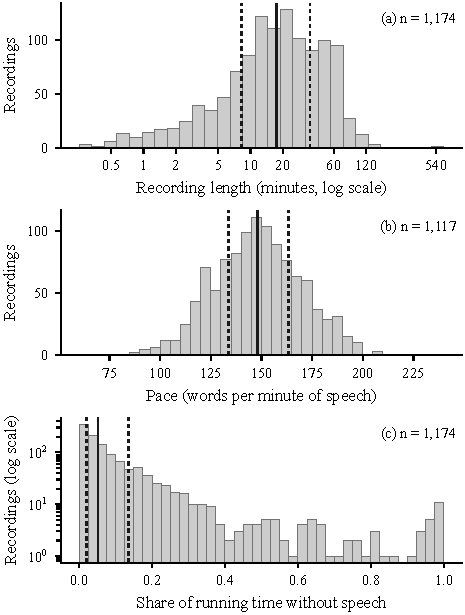
\includegraphics[width=0.8\columnwidth]{findings/fig1_distributions.pdf}
\caption{Distributions over recordings at the snapshot of \SnapDate{} (provisional): (a) recording length, (b) pace of English recordings with at least one minute of speech, (c) share of the running time without speech. Recordings of the \SnapCreatorsFivePlus{} creators with five or more finished transcripts ($n = \SeenAudio$ distinct audio files; $n = \SeenPaceN$ in b). Solid line: median; dashed lines: quartiles. The horizontal axis of (a) and the vertical axis of (c) are logarithmic. No transcript was checked by a person, and recognizer artefacts had not been removed.}
\label{fig:distributions}
\end{figure}

\subsection{Calendar, language and extension samples}

Timing analyses use exact-day dates or short intervals, compare creators only inside calendar spans that they share, and fix dates, events and word lists before any text is read (R10). \expid{EV} first publishes a feasibility table for \EvEvents{} dated outside events and as many placebo word lists, frozen by a person outside the project, and continues only if at least \EvGate{} events have enough creators posting on both sides. \expid{SY} compares recordings by different creators uploaded at most \SyNearDays{} days apart with pairs \SyFarDaysMin{} to \SyFarDaysMax{} days apart, after removing date words, against a reference that permutes upload dates within each creator. \expid{LG} places each non-English creator as a percentile among the English creators on \LgMeasures{} language-free measures, with no test (R11), and reads only measures that \expid{BR} has shown to be safe across the two models; translated text is used only where stated \cite{devries2018longer,vanmassenhove2021machine}.

Three extensions need new data. The \emph{replication wave} (\expid{RW}) is what each creator uploads after the listing of \ListingDate, collected on one later date fixed in advance (proposed: \ReplicationDate), up to \NPerCreator{} recordings per creator, through the same pipeline and one recognizer model. The \emph{comparison set} (\expid{CS}) is about \NComparisonCreators{} creators who make no channelling claim, in three strata (sermons, wellness talks, interviews), with the newest \NPerCreator{} recordings each; its selection rule and roster are frozen before any text is read, and differences are judged against an equivalence margin so that ``no difference'' can be a finding. \emph{Selection sensitivity} (\expid{SL}) recomputes each headline value under three weightings. The bridge, the replication wave and the comparison set are approved for collection; none has been collected.

\subsection{Registry and hold-out}

One registry was frozen on \RegistryFrozenDate, before any transcript of a hold-out creator was analysed for a hypothesis: \NMaxConfirmatory{} confirmatory hypotheses, each with its direction, estimand, reference distribution, threshold and refuting result, identified by a hash of the text. The procedure of each hypothesis (code, lexicons, prompts and model identifiers, each by hash) is frozen in a second entry before that hypothesis touches a hold-out transcript. The ten are stated in Section~\ref{sec:hypotheses}.

The hold-out is the \NHoldout{} creators that had at most three finished transcripts and at least ten recordings still to come at the snapshot (\HoldoutOutstanding{} recordings to come; \NHoldoutNotNonEnglish{} of these creators, with \HoldoutNotNonEnglishOutstanding{} recordings, are not flagged as non-English). Their pending recordings had not been transcribed when the pilots, the pattern passes and the reading were made; the \HoldoutInSnapshot{} audio files of these creators that were already finished did enter the recording-level descriptives. By \NowStamp{} the ledger held \HoldoutNowLines{} transcripts of these creators. None of the later ones has been analysed, and only counts are computed for these creators until the registry is frozen. The hold-out is a late part of the run, not a random draw, and the coverage audit must state what \NHoldoutNotNonEnglish{} creators can confirm. Confirmation rests on the hold-out together with the replication wave.

\subsection{Hypotheses}
\label{sec:hypotheses}

\begin{table*}[t]
\centering
\small
\setlength{\tabcolsep}{3pt}
\begin{tabular}{@{}l>{\raggedright\arraybackslash}p{0.325\textwidth}>{\raggedright\arraybackslash}p{0.335\textwidth}>{\raggedright\arraybackslash}p{0.07\textwidth}>{\raggedright\arraybackslash}p{0.175\textwidth}@{}}
\toprule
Id & Hypothesis and direction & Estimand and unit & Exp. & Confirmed on \\
\midrule
H1 & The claimed voice is slower than the creator's own voice in the same recording, by at least 5\% & creator mean of the within-recording log ratio of syllable rate, claimed over own spans & \expid{SG}, \expid{RH} & hold-out and wave, pooled \\
H2 & The more checkable a statement about the future, the less committed its wording (Somers' $D<0$, $|D|\geq 0.10$) & within-creator $D$ between checkability (0 to 5) and binary commitment, at fixed statement length & \expid{FL} & hold-out and wave, pooled \\
H3 & First-person singular is denser at the trimmed edges of a recording than in its middle ($U>0$, at least 0.10 log units) & creator mean of the log-ratio contrast $U$: first and last tenth against the middle six, 180 seconds cut from each end & \expid{PO} & hold-out creators \\
H4 & Fewer contractible forms are contracted in the embodied claimed voice than in the own voice, by at least 0.5 SD & creator mean of the within-recording difference in contraction share, in between-creator SD of the own voice & \expid{SG} & hold-out and wave, pooled \\
H5 & World-claim vocabulary, relative to practice vocabulary, is denser in a creator's channelled recordings than in its own-voice talks & within-creator difference of the log-ratio of two validated word groups (at least 0.4) & \expid{CX}, \expid{GB} & hold-out and wave, pooled \\
H6 & Asks to buy or enrol are rarer in the claimed voice than in the own voice (rate ratio at most 0.5) & creator-level within-recording rate ratio of validated asks per \RatePerWords{} words; equivalent inside 0.67 to 1.5 & \expid{AK} & hold-out and wave, pooled \\
H7 & Excess similarity of creators' recordings uploaded within \SyNearDays{} days is larger in weeks with an almanac-listed date & week-class difference of near-minus-far TF-IDF cosine between creators, date words removed & \expid{SY} & replication wave \\
H8 & The contrast of H3 is larger in channelled recordings than in sermons and wellness talks (margin 0.5 SD) & standardised difference of creator-level $U$, cohort against about 40 comparison creators & \expid{CS}, \expid{PO} & comparison set \\
H9 & Creators who name the same family of beings share more content vocabulary than function-word style & same-family minus different-family similarity between creators: content minus style, names masked & \expid{SV} & hold-out against seen creators, then wave \\
H10 & Dated forecasts whose date has passed are returned to less often than matched undated ones (conditional) & within-creator risk difference of any later reference (at least 0.15), from a ledger frozen before the wave & \expid{FL}, \expid{RW} & replication wave \\
\bottomrule
\end{tabular}
\caption{Registry of confirmatory hypotheses, frozen on \RegistryFrozenDate. H3 has been tested and withdrawn from the claims (Section~\ref{sec:hthree}); the other nine have not been run. The creator is the unit throughout; thresholds are the smallest effects of interest adopted at the freeze. ``Claimed voice'': spans that a creator presents as a channelled or relayed voice, marked from the verbal framing with timing hidden; ``embodied'': the being is voiced in the first person. ``Wave'': the replication wave, later recordings of the same roster. H10 runs only if 50 dated statements from 15 creators have matured. Experiments as in Tables~\ref{tab:expA} and~\ref{tab:expB}.}
\label{tab:hypotheses}
\end{table*}

Table~\ref{tab:hypotheses} states the registry of \NMaxConfirmatory{} hypotheses as it was frozen on \RegistryFrozenDate. One of them, H3, has been tested (Section~\ref{sec:hthree}); for the other nine no hold-out transcript has been analysed. Two proposers wrote 24 proposals, and a skeptic judged each and searched again for prior work. Ten were kept with changes, thirteen stay exploratory and one was merged. Each candidate has a direction, a creator-level estimand built from a contrast within a recording or a creator, a reference distribution, a smallest effect of interest and a result that refutes it; each was kept only if either outcome would be informative.

\paragraph{Voice.} H1 and H4 compare what a creator presents as a being's voice with the creator's own voice in the same recording. The one laboratory study reports voice differences when a story is read in both states \cite{wahbeh2019physiological}; we have not verified a reading-time result in it, so H1 is a field test, not a replication. The formality of ritual and trance speech is long described \cite{irvine1979formality,keane1997religious,hughes1991blending}; H4 asks how large it is against the spread between speakers. H5 and H6 ask what the claimed voice is used for: claims about the world \cite{hammer2001claiming} and asks to buy, which published work classifies by channel or video \cite{hua2022characterizing,ballard2022conspiracy}. H1, H4 and H6 need spans marked from the creator's verbal framing, with timing hidden, because states cut on timing (\expid{SG}) would build the contrast in; under the amended registry a language model does the marking, not two people.

\paragraph{Structure and forecasts.} H3 carries position curves from written stories \cite{boyd2020narrative} to self-reference in speech \cite{goffman1979footing}. It may still be a platform convention, which H8 tests against sermons and wellness talks. H2 carries a trade-off known from judgment research \cite{yaniv1995graininess} into prophecy, and H10 observes prospectively what the literature on failed prophecy reconstructs afterwards \cite{dawson1999prophecy,zygmunt1972prophecies}. H7 and H9 concern what creators share: calendar time \cite{leskovec2009memetracking}, and the wording of a commonly claimed source, compared so far across three speakers \cite{wahbeh2026semantic}.

\paragraph{What can be confirmed.} Only H3 could run on the hold-out without labels, and it has been run. Out-of-sample evidence at creator level comes only from the \NHoldoutNotNonEnglish{} English hold-out creators; the wave holds later recordings of the same roster and shows persistence. Counting signs, eight creators must all agree to pass the first Holm step among \NMaxConfirmatory, and twelve tolerate one dissenter; H1, H4 and H6 therefore pool hold-out and wave and are not run below twelve creators. H8 needs about 40 comparison creators, or a margin near 0.8 standard deviations, to reach a verdict. A measurement gate outside the registry asks whether the recognizer's inserted phrase follows the decoding window or silence. Novelty statements rest on the skeptic's 147 keyword searches (99 Crossref, 48 arXiv) and the proposers' searches; they mean not found, never absent.

\subsection{Bridge between the two recognizer models}
\label{sec:bridge}

English was transcribed by an English-only model and the other languages by a larger multilingual one, so no English recording had been through both. After the run, \BridgePairs{} English recordings (one per creator, drawn by seed over thirds of pace and of time without speech, hold-out creators excluded) were transcribed again by the larger model; none failed a check. For \BridgeMeasures{} measures we report the mean paired difference in units of the standard deviation between creators, taken from \BridgeSpreadCreators{} seen creators. The rule was fixed in the catalogue beforehand: a measure may be compared across the models only if the 90\% interval of the difference lies inside \BridgeMargin{} of that spread.

\BridgeAgree{} measures agree: speaking pace, the rates of first-person singular, first-person plural and second-person forms, contracted forms, the variety of words and their length in letters. \BridgeDiffer{} differ, with the whole interval outside the margin: the larger model gives words \BridgeWordMs{} milliseconds more length, about half as many pauses of 0.3 to 1 second (\BridgeShortPauseSd{} standard deviations), fewer long pauses, a smaller share of time in pauses, longer segments, and \BridgeFillerRatio{} times as many filled pauses (\BridgeFillerLarge{} against \BridgeFillerSmall{} per 1{,}000 words). \BridgeOpen{} measures, all of them rates of recognizer artefacts or confidence, are not settled by \BridgePairs{} recordings. The two transcripts of a recording differ in \BridgeDisagreeMedian\% of words at the median (quartiles \BridgeDisagreeLow\% and \BridgeDisagreeHigh\%); neither is a human reference, so this is disagreement between models and not an error rate.

Two consequences follow. Comparisons across languages may read word-based measures and no measure of timing inside the utterance. And a count of filled pauses, or a split of tempo into pausing and articulation, describes the recognizer as much as the speaker: such measures are used inside one model only.

\subsection{First registered test: H3}
\label{sec:hthree}

H3 needs no labels, so it was run first. Its procedure was frozen by hash before any hold-out transcript was read: English recordings transcribed by the English-only model, \HThreeTrimSeconds{} seconds removed from each end, at least ten minutes and 800 words left, ten equal parts each with 50 words or more, the recognizer's artefacts filtered, and the contrast $U$ between the first and last part and the middle six. The reference distribution shifts each recording's ten parts by a random offset; the interval resamples creators and then recordings.

On the hold-out, \HThreeCreators{} creators and \HThreeRecordings{} recordings were eligible. $U$ is \HThreeU{} (90\% interval over creators \HThreeLo{} to \HThreeHi), the one-sided shift test gives $p=\HThreeP$, and \HThreePositive{} of the \HThreeCreators{} creators have a positive $U$. By the registered rule ($p\leq 0.005$ and $U\geq 0.10$) H3 is supported. We do not claim it, for three reasons. The interval over creators includes zero, and a few creators with a large contrast carry the mean. The \HThreeSeenCreators{} creators seen earlier (\HThreeSeenRecordings{} recordings; exploratory) give $U=\HThreeSeenU$ (\HThreeSeenLo{} to \HThreeSeenHi; $p=\HThreeSeenP$). And the shift test asks whether position matters in these recordings at all; it does not count the differences between creators as uncertainty, which rule R1 requires. Counted before the test, the hold-out could detect a $U$ of about \HThreeDetectable{} with 80\% power, so it could not have returned a clear answer for an effect near the smallest effect of interest.

Without the trim the contrast is large in both samples (\HThreeUntrimmed{} on the hold-out, \HThreeSeenUntrimmed{} on the seen creators; reported, not tested): the surplus of first-person singular sits in the first and last three minutes, where greetings, introductions and closing words are. This is a description of how recordings open and close, not evidence about the channelled part.

\paragraph{What followed.} H3 was withdrawn from the claims of this paper after its result was seen; it keeps its row in the table of results, and it will not be tested again as a confirmatory hypothesis. H8, which compares the same contrast with sermons and wellness talks, stays registered, and whether it keeps its place is open. Three amendments to the registry are in force for the nine hypotheses not yet run. First, labels (spans of a claimed voice, forecasts, asks, sentence codes) come from prompts to a language model and not from two human markers; results that rest on them are called model-coded, no person has validated them, and their reliability is reported as agreement between two models and stability across repeated runs, which is not validity \cite{chan2021four,teblunthuis2023misclassification}. Second, hypotheses whose results are uninformative leave the claims but keep a row in the table of results, and the paper states how many were tested. Third, made after H3 and in the stricter direction: a hypothesis is called supported only if its registered test passes and the 90\% interval over creators excludes zero.

\subsection{Statistics}

Intervals come from resampling creators and then recordings within a creator (R1). Tests, where the registry allows them, use permutation or shift references with $p = (b+1)/(m+1)$ \cite{phipson2016permutation} and Holm correction across the registry; the false-discovery rate is used only as a screen. Counts are modelled with a creator intercept and a log-words offset. Claims of no difference are made by two one-sided tests against a margin stated beforehand. Shares of a whole are analysed as log-ratios and never correlated raw \cite{aitchison1982statistical,lovell2015proportionality}. Each headline is rerun under the alternatives of R8, as a specification curve whose choices are labelled \cite{simonsohn2020specification,delgiudice2021traveler,linde2026making}; figures show dots on a common scale with intervals \cite{cleveland1984graphical}.

\section{Preliminary findings}
\label{sec:findings}

All numbers in this section are provisional. Unless a sentence says otherwise they describe the \snap, taken at about 13:00 UTC while the run was still going. Three other bases occur: pattern passes over \ArtBase{} finished transcripts (artefacts, term families), a pilot on \VpLedger{} (window-level variance, correlations inside a recording), and a count on \ModelCountBase{} (recognizer model). No artefact filter has been applied, and the pilot and pattern code has not been reviewed. Everything is exploratory: we give estimates and intervals and no $p$-values. Figures~\ref{fig:distributions}, \ref{fig:variance}, \ref{fig:pace} and~\ref{fig:running} use only the \SnapCreatorsFivePlus{} creators with five or more finished transcripts. Tables~\ref{tab:descriptives} and~\ref{tab:variance} were computed before the hold-out was declared and include \LowCountInSnapshot{} audio files of creators with fewer than five transcripts, \HoldoutInSnapshot{} of them from hold-out creators.

% Generated by work2/split_floats.py from findings/tables.tex (table tab:variance). Do not edit: edit the source and re-run.
\begin{table}[t]
\centering
\small
\setlength{\tabcolsep}{4pt}
\begin{tabular}{@{}>{\raggedright\arraybackslash}p{0.46\columnwidth}rrrr@{}}
\toprule
Measure (recording level) & Cr. & Rec. & ICC & $n_{\mathrm{eff}}$ \\
\midrule
Lexical variety (MATTR-500) & \IccMattrCreators & \IccMattrRecordings & \IccMattr & \NeffMattr \\
Pace & \IccPaceCreators & \IccPaceRecordings & \IccPace & \NeffPace \\
Share of time without speech & \IccNonSpCreators & \IccNonSpRecordings & \IccNonSp & \NeffNonSp \\
Mean segment log-probability & \IccLogpCreators & \IccLogpRecordings & \IccLogp & \NeffLogp \\
Length (log minutes) & \IccLenCreators & \IccLenRecordings & \IccLen & \NeffLen \\
Share of segments ending in a question mark & \IccQuestCreators & \IccQuestRecordings & \IccQuest & \NeffQuest \\
Repeated five-word share & \IccRepCreators & \IccRepRecordings & \IccRep & \NeffRep \\
\bottomrule
\end{tabular}

\vspace{0.6em}
\begin{tabular}{@{}>{\raggedright\arraybackslash}p{0.46\columnwidth}rrr@{}}
\toprule
Measure (window level, pilot) & Creator & Rec. & Within \\
\midrule
Articulation rate (log) & \VpArtCreator & \VpArtRecording & \VpArtWithin \\
Pause-time share & \VpPauseCreator & \VpPauseRecording & \VpPauseWithin \\
Segment log-probability & \VpSegCreator & \VpSegRecording & \VpSegWithin \\
\bottomrule
\end{tabular}
\caption{Share of variance between creators. Top: one-way intraclass correlation, ICC(1), over creators (Cr.) with two or more recordings (Rec.) that hold at least one minute of speech, at the snapshot of \SnapDate{} (\SnapLines{} transcripts; provisional). $n_{\mathrm{eff}}$ is the number of recordings divided by the design effect $1 + (\bar{m} - 1)\,\mathrm{ICC}$, where $\bar{m}$ is the mean number of recordings per creator. Bottom: shares of variance between creators, between recordings of one creator and within a recording, from a pilot on \VpLedger{} transcripts (\VpCreators{} creators, \VpRecordings{} recordings, \VpArtWindows{} windows; \VpSegWindows{} for log-probability) whose code was not reviewed. Intervals for the top panel are in Figure~\ref{fig:variance}.}
\label{tab:variance}
\end{table}


\paragraph{Recordings of one creator resemble each other.} The creator accounts for \IccMinPct\% to \IccMaxPct\% of the variance of seven recording-level measures (Table~\ref{tab:variance}, Figure~\ref{fig:variance}): lexical variety \IccMattr, pace \IccPace, share of time without speech \IccNonSp, mean log-probability \IccLogp, length \IccLen, question share \IccQuest{} and repeated five-word share \IccRep{} (lexical variety is the moving-average type-token ratio over 500-word windows). For pace, the \IccPaceRecordings{} recordings carry the information of about \NeffPace{} independent ones. Restricted to the \SnapCreatorsFivePlus{} creators with five or more transcripts, the estimate for pace is \IccPaceSeen{} with a 95\% bootstrap interval of \IccPaceSeenLo{} to \IccPaceSeenHi. The intervals for share without speech (\IccNonSpSeenLo{} to \IccNonSpSeenHi), log-probability (\IccLogpSeenLo{} to \IccLogpSeenHi) and repeated five-word share (\IccRepSeenLo{} to \IccRepSeenHi) are wide, so those three shares are poorly determined. In the pilot, the variance of articulation rate splits into \VpArtCreator{} between creators, \VpArtRecording{} between recordings of one creator and \VpArtWithin{} within a recording; window-level and recording-level shares are not comparable with each other. Creator medians of pace run from \CrPaceMin{} to \CrPaceMax{} words per minute of speech (Figure~\ref{fig:pace} in the appendix).

\begin{figure}[t]
\centering
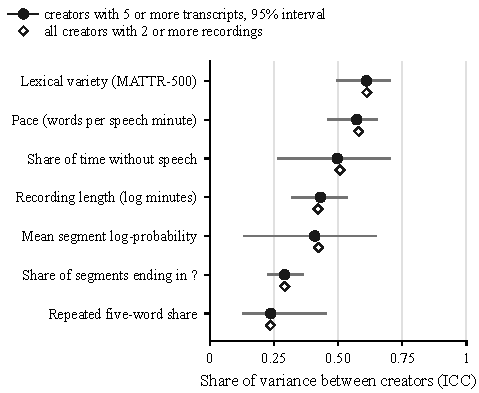
\includegraphics[width=0.8\columnwidth]{findings/fig3_variance_between_creators.pdf}
\caption{Share of variance between creators, ICC(1), for seven recording-level measures (snapshot of \SnapDate, provisional). Filled circles: creators with five or more finished transcripts (\IccSeenCreatorsMin{} to \IccSeenCreatorsMax{} creators, \IccSeenRecordingsMin{} to \IccSeenRecordingsMax{} recordings), with 95\% percentile intervals from \NBootstrap{} resamples of creators. Open diamonds: all creators with two or more recordings (\IccCreatorsMin{} to \IccCreatorsMax{} creators; Table~\ref{tab:variance}). The interval procedure has not been through the planned coverage audit.}
\label{fig:variance}
\end{figure}

\paragraph{The recordings differ widely in form.} The median recording lasts \LenMed{} minutes (quartiles \LenQi{} and \LenQiii; maximum \LenMax) and holds \WordsMed{} words. \NLenUpToFive{} recordings are five minutes or shorter and \NLenOverSixty{} are longer than an hour. The median pace of English recordings is \PaceMed{} words per minute of speech, with quartiles \PaceQi{} and \PaceQiii{} (Table~\ref{tab:descriptives}, Figure~\ref{fig:distributions}).

\paragraph{About one eighth of the audio holds no speech.} Of \SnapHours{} audio hours, \SnapNonSpeechHours{} (\SnapNonSpeechPct\%) hold no speech according to the recognizer's voice detector, and five creators hold \NonSpTopFivePct\% of that time. \NHalfNonSpeech{} recordings are at least half without speech and \NUnderFiftyWords{} hold fewer than 50 words. Stretches of 30 seconds or more without speech total \QuietHours{} hours in \NQuietRecordings{} recordings. Speech is thinner at the ends of a recording: it covers \CovFirst{} of the first tenth of the running time, \CovMiddle{} in the middle and \CovLast{} of the last tenth (Figure~\ref{fig:running} in the appendix).

\paragraph{Recognizer confidence follows delivery.} Across \RhoN{} English recordings the mean segment log-probability rises with pace (Spearman \RhoLogpPace) and falls with the share of time without speech (\RhoLogpNonSp); it is unrelated to length (\RhoLogpLen). Across the \SnapCreatorsFivePlus{} creator medians the correlation with pace is \RhoCreatorLogpPace. Inside a recording the picture differs: in the pilot, over \RhoWithinRecordings{} recordings of \RhoWithinCreators{} creators, which include creators outside the \SnapCreatorsFivePlus, the correlation between segment log-probability and segment pace has a median of \RhoWithinMed{} and is positive in \RhoWithinPositivePct\% of recordings. A commonly used stock cut-off of \StockLogpCutoff, which we did not confirm in the recognizer paper, flags almost nothing: the share of segments below it is \ShareBelowCutoffMed{} at the median and \ShareBelowCutoffPninetyfive{} at the 95th percentile. We treat log-probability as a covariate and not as a quality score until it has been calibrated against hand transcripts.

% Generated by work2/split_floats.py from findings/tables.tex (table tab:artefacts). Do not edit: edit the source and re-run.
\begin{table}[t]
\centering
\small
\begin{tabular}{@{}>{\raggedright\arraybackslash}p{0.52\columnwidth}rr@{}}
\toprule
Artefact & Segments & Transcripts \\
\midrule
Inserted two-word thanks phrase & \ThanksSegments & \ThanksTranscripts{} (\ThanksPct\%) \\
\quad starting 27 to 30\,s into a decoding window & \ThanksLateWindow{} (\ThanksLateWindowPct\%) & \\
\quad with under 1\,s of gap on both sides & \ThanksEmbedded{} (\ThanksEmbeddedPct\%) & \\
Isolated segment of at most three words, 5\,s of silence on both sides & \IsoSegments & \IsoTranscripts{} (\IsoPct\%) \\
\quad starting on a multiple of 30\,s & \IsoGridPct\% & \\
Segment with compression ratio above 2.4 & \LoopSegments & \LoopTranscripts{} (\LoopPct\%) \\
\midrule
Stored non-speech value of zero & & \ZeroNonSpeech{} of \ArtBase \\
Fewer than 50 words & & \NUnderFiftyWords{} of \SnapAudio \\
At least half of the running time without speech & & \NHalfNonSpeech{} of \SnapAudio \\
\bottomrule
\end{tabular}
\caption{Recognizer artefacts found by pattern rules, with no audio played and no human reference. Rows above the rule: \ArtEnglishBase{} English transcripts (\ArtSegmentBase{} segments) among the \ArtBase{} finished when the reading pass ran on \SnapDate; percentages in the last column are of those transcripts. The last two rows are from the snapshot of \SnapLines{} transcripts. Counts come from unreviewed code and are provisional; the rules have not been checked against listening.}
\label{tab:artefacts}
\end{table}


\paragraph{Recognizer artefacts are frequent and tied to the decoding window.} In \ArtEnglishBase{} English transcripts a two-word thanks phrase stands alone as a segment \ThanksSegments{} times, in \ThanksTranscripts{} transcripts (\ThanksPct\%). \ThanksLateWindowPct\% of these segments start 27 to 30 seconds into a \WindowSeconds-second decoding window, and \ThanksEmbeddedPct\% sit in running speech with under a second of gap on both sides; their median log-probability is \ThanksLogp{} against \OtherShortLogp{} for other short segments. A further \IsoSegments{} isolated segments of at most three words sit in silence or music in \IsoTranscripts{} transcripts (\IsoPct\%), \IsoGridPct\% of them starting exactly on a multiple of \WindowSeconds{} seconds (Table~\ref{tab:artefacts}). In the reading sample a single name was spelt in \SpellingsMin{} to \SpellingsMax{} ways inside one recording. No audio was played for these counts: a segment is called invented because it matches a known pattern and does not fit its context, and the rules have not been checked against listening.

% Generated by work2/split_floats.py from findings/tables.tex (table tab:kinds). Do not edit: edit the source and re-run.
\begin{table}[t]
\centering
\small
\begin{tabular}{@{}>{\raggedright\arraybackslash}p{0.78\columnwidth}r@{}}
\toprule
Kind of recording (read sample, 300 words or more) & $n$ \\
\midrule
Channelled voice or relayed message & \KindChannelled \\
Interview or podcast without channelling & \KindInterview \\
Guided meditation & \KindMeditation \\
Talk in the creator's own voice & \KindOwnVoice \\
Other kinds & \KindOther \\
\midrule
Total & \ReadLongN \\
\bottomrule
\end{tabular}

\vspace{0.6em}
\begin{tabular}{@{}>{\raggedright\arraybackslash}p{0.78\columnwidth}r@{}}
\toprule
Term family present in the transcript & Share \\
\midrule
Soul & \TermSoul\% \\
Frequency or vibration & \TermFrequency\% \\
Breath & \TermBreath\% \\
Ascension & \TermAscension\% \\
Any extraterrestrial or alien word & \TermExtraterrestrial\% \\
\bottomrule
\end{tabular}
\caption{Top: kinds of recording among the \ReadLongN{} read recordings with 300 words or more. The \ReadN{} read recordings (\ReadCreators{} creators) were chosen by stratum for contrast, not at random, and one reader assigned the kinds, so the counts do not estimate corpus shares. Bottom: share of \TermBase{} English transcripts of 150 words or more that contain a term family, from crude regular expressions over the \ArtBase{} transcripts finished on \SnapDate; the lists were not validated and misrecognized words lower the counts. Both panels are provisional.}
\label{tab:kinds}
\end{table}


\paragraph{A recording filed under a channeler is often not channelled speech.} \ReadN{} finished transcripts from \ReadCreators{} creators were read by one reader, \ReadFull{} of them in full; they were chosen by stratum for contrast and not at random. Of the \ReadLongN{} with 300 words or more, \KindChannelled{} hold a channelled voice or a relayed message. The others are interviews or podcasts without channelling (\KindInterview), guided meditations (\KindMeditation), talks in the creator's own voice (\KindOwnVoice), a hypnosis session and an event advertisement (Table~\ref{tab:kinds}). The reader noted \NSpeakingModes{} speaking modes, among them a being voiced in the first person, a relay in the creator's own voice and a scripted persona read without pauses. Only \ReadAudienceQA{} of the \ReadN{} read recordings hold audience questions and answers, so the share of segments that end in a question mark (median \QuestMed) does not measure audience questions. The sample shows that these kinds exist, not how common they are.

\paragraph{Extraterrestrial vocabulary is a minority register.} Among \TermBase{} English transcripts of 150 words or more, \TermSoul\% contain a soul term, \TermFrequency\% a frequency or vibration term, \TermBreath\% a breath term and \TermAscension\% an ascension term, against \TermExtraterrestrial\% with any extraterrestrial or alien word. The patterns are crude regular expressions that no one has validated, and misrecognized words lower the counts; the shares are orders of magnitude.

\paragraph{The newest \NPerCreator{} recordings are a quota, not a period.} The window covered by a creator's newest \NPerCreator{} recordings spans \SpanMin{} to \SpanMax{} days (median \SpanMed; quartiles \SpanQi{} and \SpanQiii): \NSpanWithinMonth{} creators fit inside 30 days and \NSpanOverTwoYears{} need more than two years. \PctDatedCaptureYear\% of the \NSelected{} selected recordings are dated in the year of capture and \PctDatedYearBefore\% in the year before. Order within a creator is not time across creators, and an upload date is not the date of speaking, so the cohort supports no trend claim.

\paragraph{Language.} At the snapshot \SnapNonEnglish{} audio files from \SnapNonEnglishCreators{} creators are in a language other than English (Japanese \SnapJapanese, Spanish \SnapSpanish, Portuguese \SnapPortuguese, Czech \SnapCzech; \NowNonEnglish{} files from \NowNonEnglishCreators{} creators in the ledger at \NowStamp), so a language here means one or two creators, a different recognizer model and a translation step at once.

\section{Discussion and limitations}
\label{sec:limits}

\paragraph{What the first numbers change in the design.} Four findings constrain everything that follows. The creator carries \IccMinPct\% to \IccMaxPct\% of the variance, so the sample for inference is about a hundred creators. Recognizer confidence follows pace and silence between creators and behaves differently inside a recording, so it cannot serve as a quality filter: dropping low-confidence text would drop slow, music-backed recordings. Only \KindChannelled{} of the \ReadLongN{} longer recordings read held channelled speech, so content statistics need a part-of-recording label first, and that label needs human boundaries. And the recognizer's inserted phrase is itself a phrase of thanks, so counts of thanks, closings and short answers are unusable until the filter is applied and checked.

\paragraph{Limitations.} The following limits apply to every statement in this paper.
\begin{itemize}
\item \emph{Quota sample of a purposive roster.} The creators were chosen by the authors, and the newest \NPerCreator{} recordings of each cover from \SpanMin{} days to \SpanMaxYears{} years. Nothing here describes channelers at large, a period, or a history.
\item \emph{Single platform.} Selection used one platform's listing of regular uploads; short-form video, live streams and other platforms are outside the cohort, and \NFailed{} selected recordings have no audio.
\item \emph{Unfinished run.} The snapshot covers \SnapPctAudio\% of the audio files and \SnapPctHours\% of the hours, and the remainder is not random: of \SnapNotInLedger{} recordings then outstanding, \SnapNotInLedgerConcentrated{} belong to \SnapNotInLedgerCreators{} creators.
\item \emph{No measured recognition error.} All transcripts are unreviewed, and recognizer confidence is not accuracy. Word time stamps, the split into speech and non-speech and every word count carry unmeasured error; names are the least reliable words. No artefact filter has been applied, and the artefact counts come from unreviewed pattern rules.
\item \emph{No speakers, no comparison set.} Host, guest, audience, the creator's own voice and a channelled voice are one stream, so no number is per channelled word. With no corpus of non-channelling speech, nothing reported can be called distinctive of channelling.
\item \emph{Few non-English creators and two models.} Other languages come from \SnapNonEnglishCreators{} creators at the snapshot (\NowNonEnglishCreators{} in the ledger at \NowStamp). Language, creator, recognizer model and translation cannot be separated. The bridge (Section~\ref{sec:bridge}) allows pace, pronoun and vocabulary measures to be read across the two models, and no measure of pauses or fillers.
\item \emph{One reader, purposive sample.} The kinds of recording rest on one reader and \ReadN{} recordings chosen for contrast, with no second coder and no segment labels.
\item \emph{Hold-out.} The \NHoldout{} hold-out creators are those the run reached last, not a random draw; \HoldoutInSnapshot{} of their audio files entered the recording-level tables before the hold-out was declared; and the report on the finished run tabulates duration, word count, language and the share of audio without speech for every recording, the hold-out included. No text of a hold-out transcript was analysed for a hypothesis before that hypothesis's procedure was frozen. The hold-out is small: \HThreeCreators{} creators were eligible for the one test run so far, which could detect only an effect of about \HThreeDetectable{} log units.
\item \emph{Intervals and literature.} The intervals shown are percentile bootstrap intervals whose coverage has not been audited. The literature studies used automated extraction and abstract-level search; we cite arXiv versions, which can differ from proceedings versions, and report no number from a cited paper.
\end{itemize}

\paragraph{Next steps.} When the run closes, every number in Section~\ref{sec:findings} is recomputed and the artefact filter is applied. The registry is frozen before any transcript of a hold-out creator is analysed, and the hand-reference study comes before every experiment that uses a word list, a label or a boundary.

\section{Ethics and data statement}
\label{sec:ethics}

\paragraph{Material and reporting.} The recordings are public uploads by creators who address a public audience. Public availability is not consent to research use, and we limit what is done with the material accordingly. The recordings and their texts belong to their makers; copies are held privately for non-consumptive analysis. This paper contains no transcript text, not even short quotations, and names no creator, channel or being; creators appear as counts or coded identifiers. Outputs of the analysis are numbers, coded identifiers and derived labels (R15), and rankings on selling, forecasts or certainty are not published by creator.

\paragraph{Individuals and claims.} The analysis describes recordings and groups of creators. It makes no statement about a creator's sincerity, mental state or health. Some recordings include audience members or clients; they are never quoted or described, and nothing about their health or circumstances is reported. We neither assert nor deny that any being speaks in these recordings: statements about the future, about healing or about hidden events are recorded as statements with no truth label.

\paragraph{Removal, review and assistance.} The rules require that every release carries a removal route, through which a creator can ask for material about their recordings to be taken down, and a datasheet \cite{gebru2018datasheets}. No ethics review decision is recorded for the project at the time of writing; one is required before paid annotators or an institution take part, which the hand-reference study may involve. The literature studies were made with an automated extractor, and this draft was prepared with an AI writing assistant from the project's documents; neither replaces checking by the authors.

\paragraph{Reproducibility.} Planned for release with the final version: the collection and transcription code with pinned model revisions and dependency hashes; the selection rule and counts by status; the experiment catalogue with its rules; the frozen registry and the hashes of its lexicons and lists; and, for every table and figure, the derived data file behind it, with creators as coded identifiers in every analysis table. Collection-status and date tables at the level of the recording hold public metadata only and are kept apart from analysis outputs. Kept private: audio, transcripts in any language, hand transcripts, embeddings of the text, single-recording timelines and example lines.

\bibliography{refs}

\appendix
\renewcommand{\thefigure}{A\arabic{figure}}
\setcounter{figure}{0}

\section{Additional figures}
\label{sec:appendix}

Figure~\ref{fig:calendar} supplements Section~\ref{sec:data}; it uses listing dates only. Figures~\ref{fig:pace} and~\ref{fig:running} supplement Section~\ref{sec:findings} and are provisional in the same sense as the numbers there.

\begin{figure}[t]
\centering
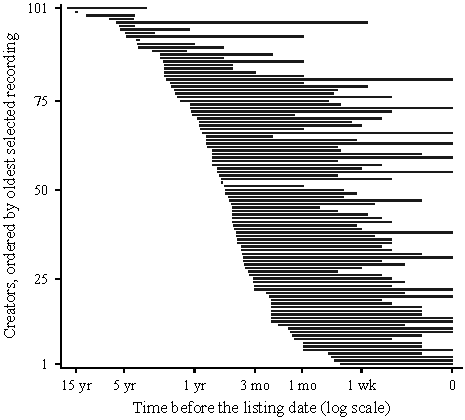
\includegraphics[width=0.8\columnwidth]{findings/figA_calendar_window.pdf}
\caption{Calendar window of the newest \NPerCreator{} recordings of each of the \NCreators{} creators: one line per creator, from its oldest to its newest selected recording, in time before the listing date of \ListingDate{} (logarithmic axis). The windows span \SpanMin{} to \SpanMax{} days (median \SpanMed). \NEstimatedDates{} of the \NSelected{} dates are intervals estimated from a displayed age, and the line uses the interval ends. Dates are upload dates, not dates of speaking. The figure uses listing dates only and no transcript.}
\label{fig:calendar}
\end{figure}

\begin{figure}[t]
\centering
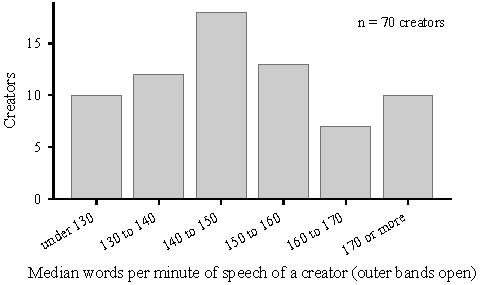
\includegraphics[width=0.8\columnwidth]{findings/fig2_creator_pace.pdf}
\caption{Median pace per creator, ranked, with 95\% intervals (snapshot of \SnapDate, provisional). \NFigTwoCreators{} creators with five or more English recordings of at least one minute of speech. Intervals are percentile intervals from \NBootstrap{} resamples of each creator's recordings. Filled marks: eight or more recordings; hollow marks: five to seven. Dashed line and band: median and interquartile range of the creator medians. Values are raw, not shrunken. The intervals are not rank intervals and their coverage has not been audited, so the figure does not single out any creator.}
\label{fig:pace}
\end{figure}

\begin{figure}[t]
\centering
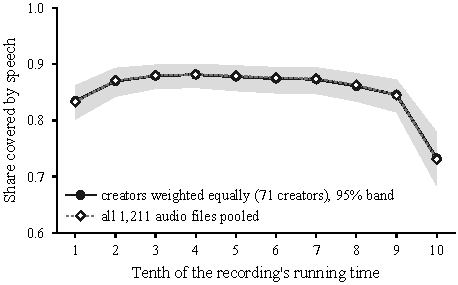
\includegraphics[width=0.8\columnwidth]{findings/fig4_speech_along_running_time.pdf}
\caption{Mean share of each tenth of a recording's running time that is covered by speech segments (snapshot of \SnapDate, provisional). Filled circles: creators weighted equally (\SnapCreatorsFivePlus{} creators with five or more finished transcripts, \SeenAudio{} audio files), with a pointwise 95\% band from \NBootstrap{} two-stage resamples (creators, then recordings). Open diamonds: all \SnapAudio{} audio files pooled. Speech segments are the output of the recognizer's voice detector and were not validated; the band is pointwise, not simultaneous.}
\label{fig:running}
\end{figure}

\end{document}
